\documentclass[12pt]{article}
\usepackage{amsmath}
\usepackage{graphicx}
\usepackage{caption}
\usepackage{float}
\usepackage[utf8]{inputenc}
\usepackage{geometry}
\usepackage{svg}
\usepackage{listings}
\usepackage{xcolor}
\usepackage{longtable}
\usepackage{polski}
\geometry{a4paper, margin=1in}

\title{Zadanie 2 z Metod Probabilistycznych i Statystyki}
\author{Mikołaj Krupiński}
\date{Grudzień 2022}

\definecolor{codegreen}{rgb}{0,0.6,0}
\definecolor{codegray}{rgb}{0.5,0.5,0.5}
\definecolor{codepurple}{rgb}{0.58,0,0.82}
\definecolor{backcolour}{rgb}{0.95,0.95,0.92}

\lstdefinestyle{mystyle}{
  backgroundcolor=\color{backcolour},   commentstyle=\color{codegreen},
  keywordstyle=\color{magenta},
  numberstyle=\tiny\color{codegray},
  stringstyle=\color{codepurple},
  basicstyle=\ttfamily\footnotesize,
  breakatwhitespace=false,         
  breaklines=true,                 
  captionpos=b,                    
  keepspaces=true,                 
  numbers=left,                    
  numbersep=5pt,                  
  showspaces=false,                
  showstringspaces=false,
  showtabs=false,                  
  tabsize=2
}

\lstset{style=mystyle}

\begin{document}

\maketitle

\section{Wprowadzenie}
Celem zadania jest przeprowadzenie losowego eksperymentu polegającego na wrzucaniu kul do $n$ jednostajnie losowo wybranych ponumerowanych urn. Będę wyznaczał następujące wielkości:
\begin{itemize}
    \item $B_n$ - moment pierwszej kolizji, tzn. pierwszy numer rzutu, w którym wylosowana kula trafiła do niepustej urny
    \item $U_n$ - liczba pustych urn po wrzuceniu $n$ kul
    \item $L_n$ - maksymalna liczba kul w urnie po wrzuceniu $n$ kul
    \item $C_n$ - minimalna liczba rzutów, po której w każdej z urn jest co najmniej jedna kula
    \item $D_n$ - minimalna liczba rzutów, po której w każdej urnie są co najmniej dwie kule
    \item $D_n - C_n$ - liczba rzutów od momentu $C_n$ potrzebna, do tego żeby w każdej urnie były co najmniej dwie kule.
\end{itemize}

\section{Generowanie losowych statystyk}

Poniższy skrypt w $Python'ie$ symuluje wrzucanie kul do jednostajnie losowo wybranych urn. Liczba testowanych urn wynosi $n \in \{1000, 2000, ..., 100000\}$. Dla każdego $n$ wykonuję $k=50$ niezależnych powtórzeń eksperymentu. Wyniki poszczególnych prób losowych zapisuję do pliku, do późniejszej analizy przez kolejny program.

\begin{lstlisting}[language=Python, caption=generate\_data.py]
import numpy as np
from random import randint
    
f = open("results.txt", "w")
    
for n in range(1000, 100000 + 1, 1000):
          
    for k in range(50):
         
        ballsInBins = np.zeros(n) # each cell stores number of balls in each bin
    
        wasConflict = False # set to True after first conflict
    
        # variables to store results for each task
        conflict_place = 0
        empty_bins_after_n = 0
        max_balls_in_bin = 0
        throws_one_ball = 0
        throws_two_balls = 0
    
        bins_less_two_balls = n # number of bins with less than two balls
        empty_bins = n # number of currently empty bins
        t = 0 # number of already thrown balls
    
        while bins_less_two_balls > 0:
            # choosing random bin to throw ball into
            selectedBin = randint(0, n - 1)
            ballsInBins[selectedBin] += 1
            t += 1
    
            # empty bin is now not empty
            if ballsInBins[selectedBin] == 1:
                empty_bins -= 1
    
            # one-ball-bin has now two balls
            if ballsInBins[selectedBin] == 2:
                bins_less_two_balls -= 1
                # check if it's not the first conflict
                if not wasConflict:
                    wasConflict = True
                    conflict_place = t
    
            # after n-th ball thrown
            if t == n:
                empty_bins_after_n = len([bin for bin in ballsInBins if bin == 0])
                max_balls_in_bin = int(np.max(ballsInBins))
                
            # first momeant when all bins are full
            if throws_one_ball == 0 and empty_bins == 0:
                throws_one_ball = t
    
        # 'while' loop has finished so all the bins have at least two balls
        throws_two_balls = t
    
                
    f.write(str(conflict_place) + ';' + str(empty_bins_after_n) + ';' + str(max_balls_in_bin) + ';'
        + str(throws_one_ball) + ';' + str(throws_two_balls) + ';' + str(throws_two_balls - throws_one_ball) + '\n')
    
f.close()
\end{lstlisting}

\section{Rysowanie wykresów}

Wykresy rysowałem za pomocą biblioteki $Matplotlib$ w języku $Python$. Dane zaimportowałem z wcześniej wygenerowanego pliku z danymi, a następnie wykonałem niezbędne obliczenia i narysowałem wykresy.



\section{Wykresy dla poszczególnych statystyk}

Na każdym z wykresów wygenerowanych dla opisanych we wstępie wielkości. Niebieskie kropki oznaczają wyniki poszczególnych z $k$ prób, a czerwone kropki średnie wartości dla każdego $n$. Ponadto dla każdej wielkości będę starał się określić asymptotykę i w tym celu narysowałem wykresy ułatwiające jej określenie. Funkcje oznaczone małymi literami oznaczają wielkości określone na początku wielkimi literami dla danego $n$, np. $b(n)$ oznacza wynik eksperymentu wyznaczającego $B_n$ dla określonego $n$.

\subsection*{Moment pierwszej kolizji}

Na wykresie $B_n$ wartości średnie układają się w linie przypominającą funkcję $\sqrt{n}$. Taką hipotezę potwierdza wykres $\frac{b(n)}{\sqrt{n}}$, który przypomina funkcję liniową. Zatem można wyciągnąć wniosek, iż $b(n)=\Theta(\sqrt{n})$. Z pierwszego z mniejszych wykresów wynika, że $b(n)=o(n)$, ponieważ wartości na wykresie zbiegają do 0. Koncentracja wokół wartości średnich maleje wraz ze wzrostem $n$, jednak trend widoczny jest już dla $n \leq 60000$.

\begin{figure}[H]
    \centering
    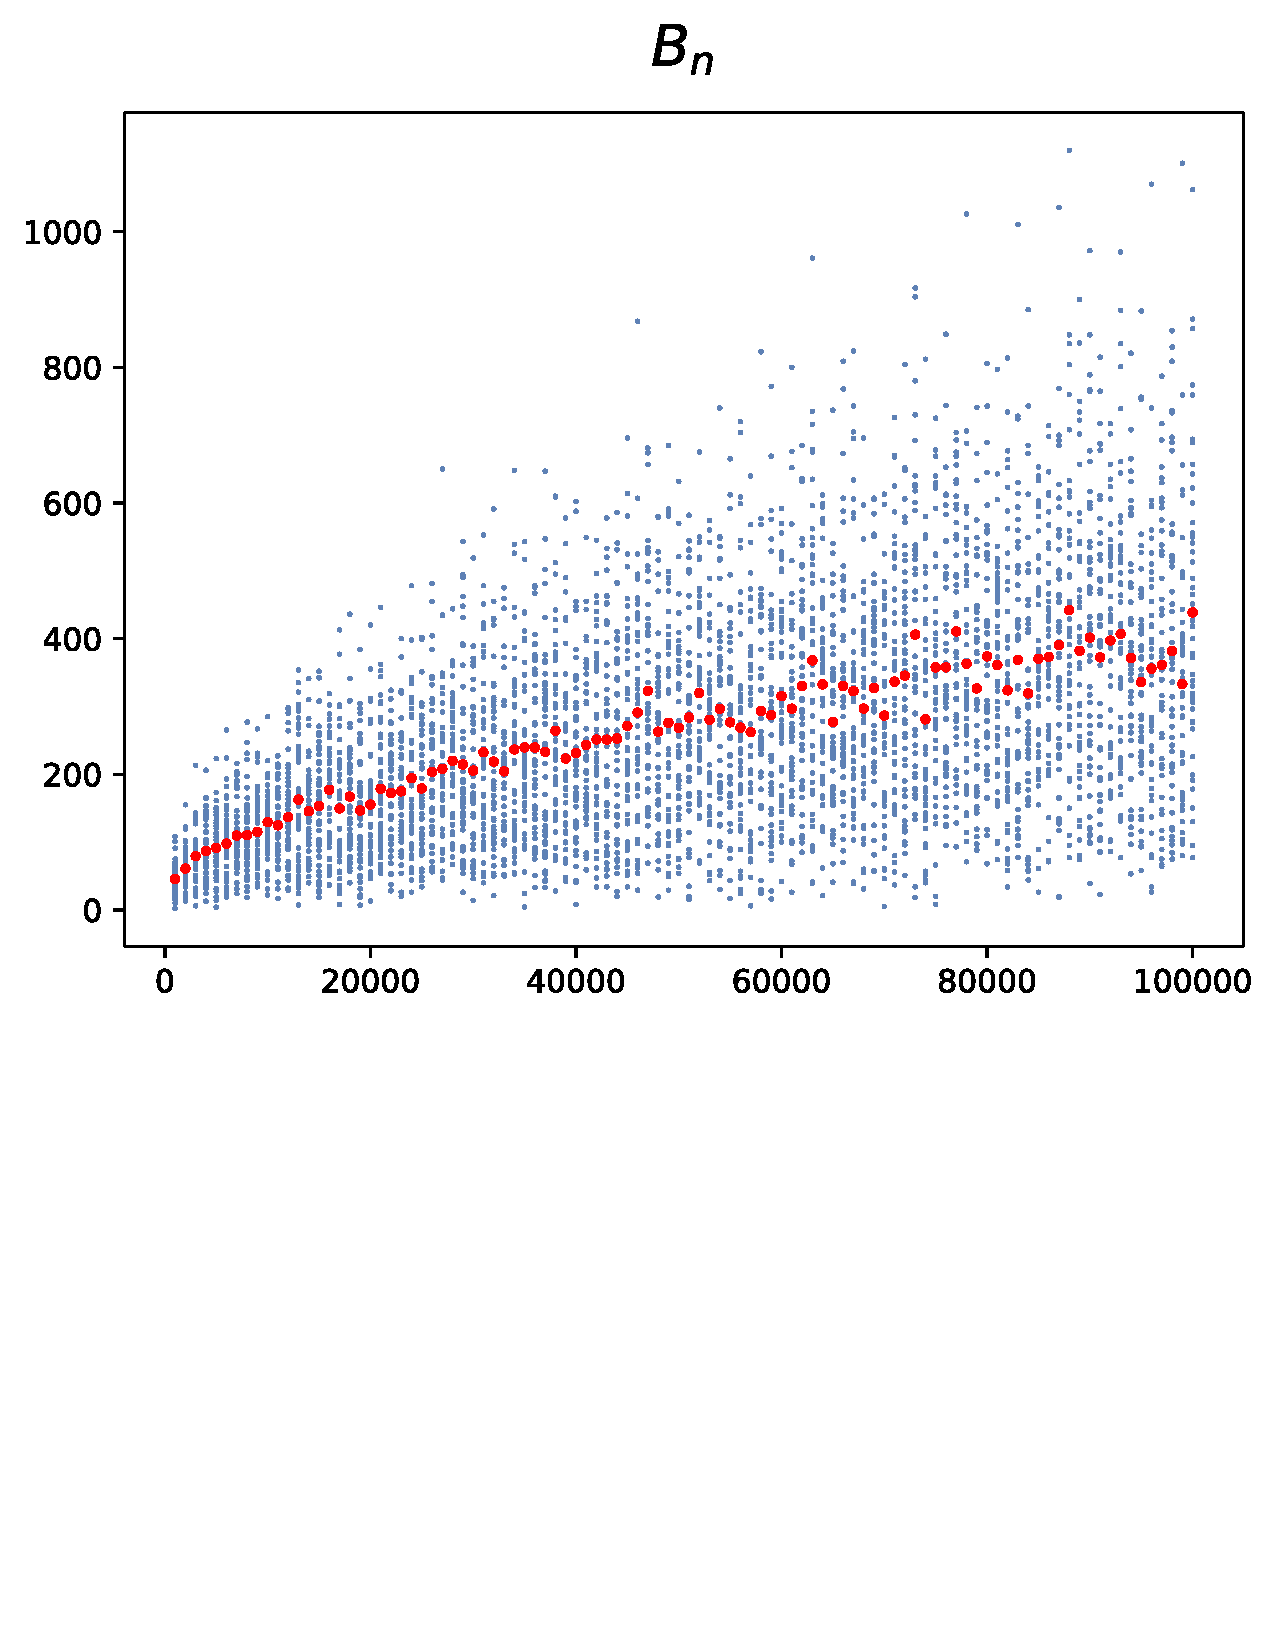
\includegraphics[width=15cm, trim = 0 11cm 0 0, clip]{images/bn.pdf}
\end{figure}
\begin{figure}[H]
    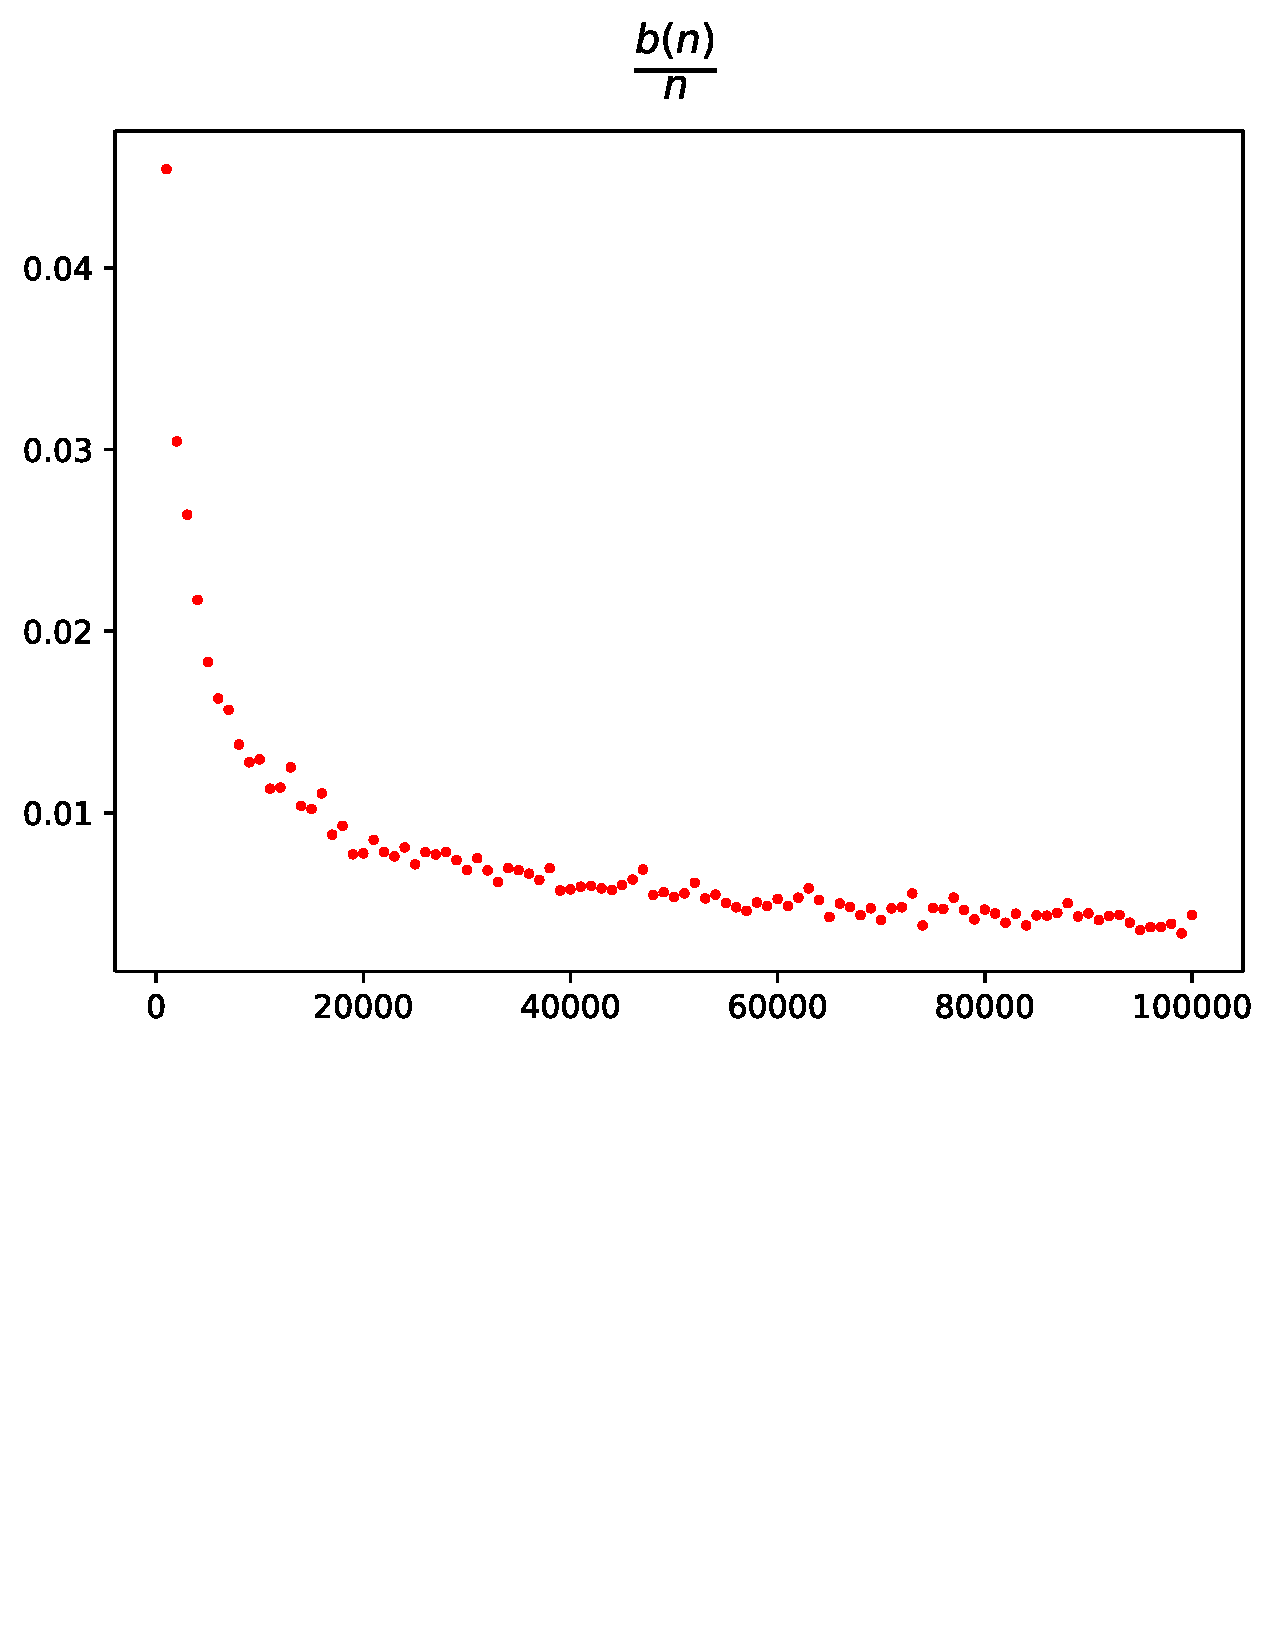
\includegraphics[width=8cm, trim = 0 10cm 0 0, clip]{images/bn1.pdf}
    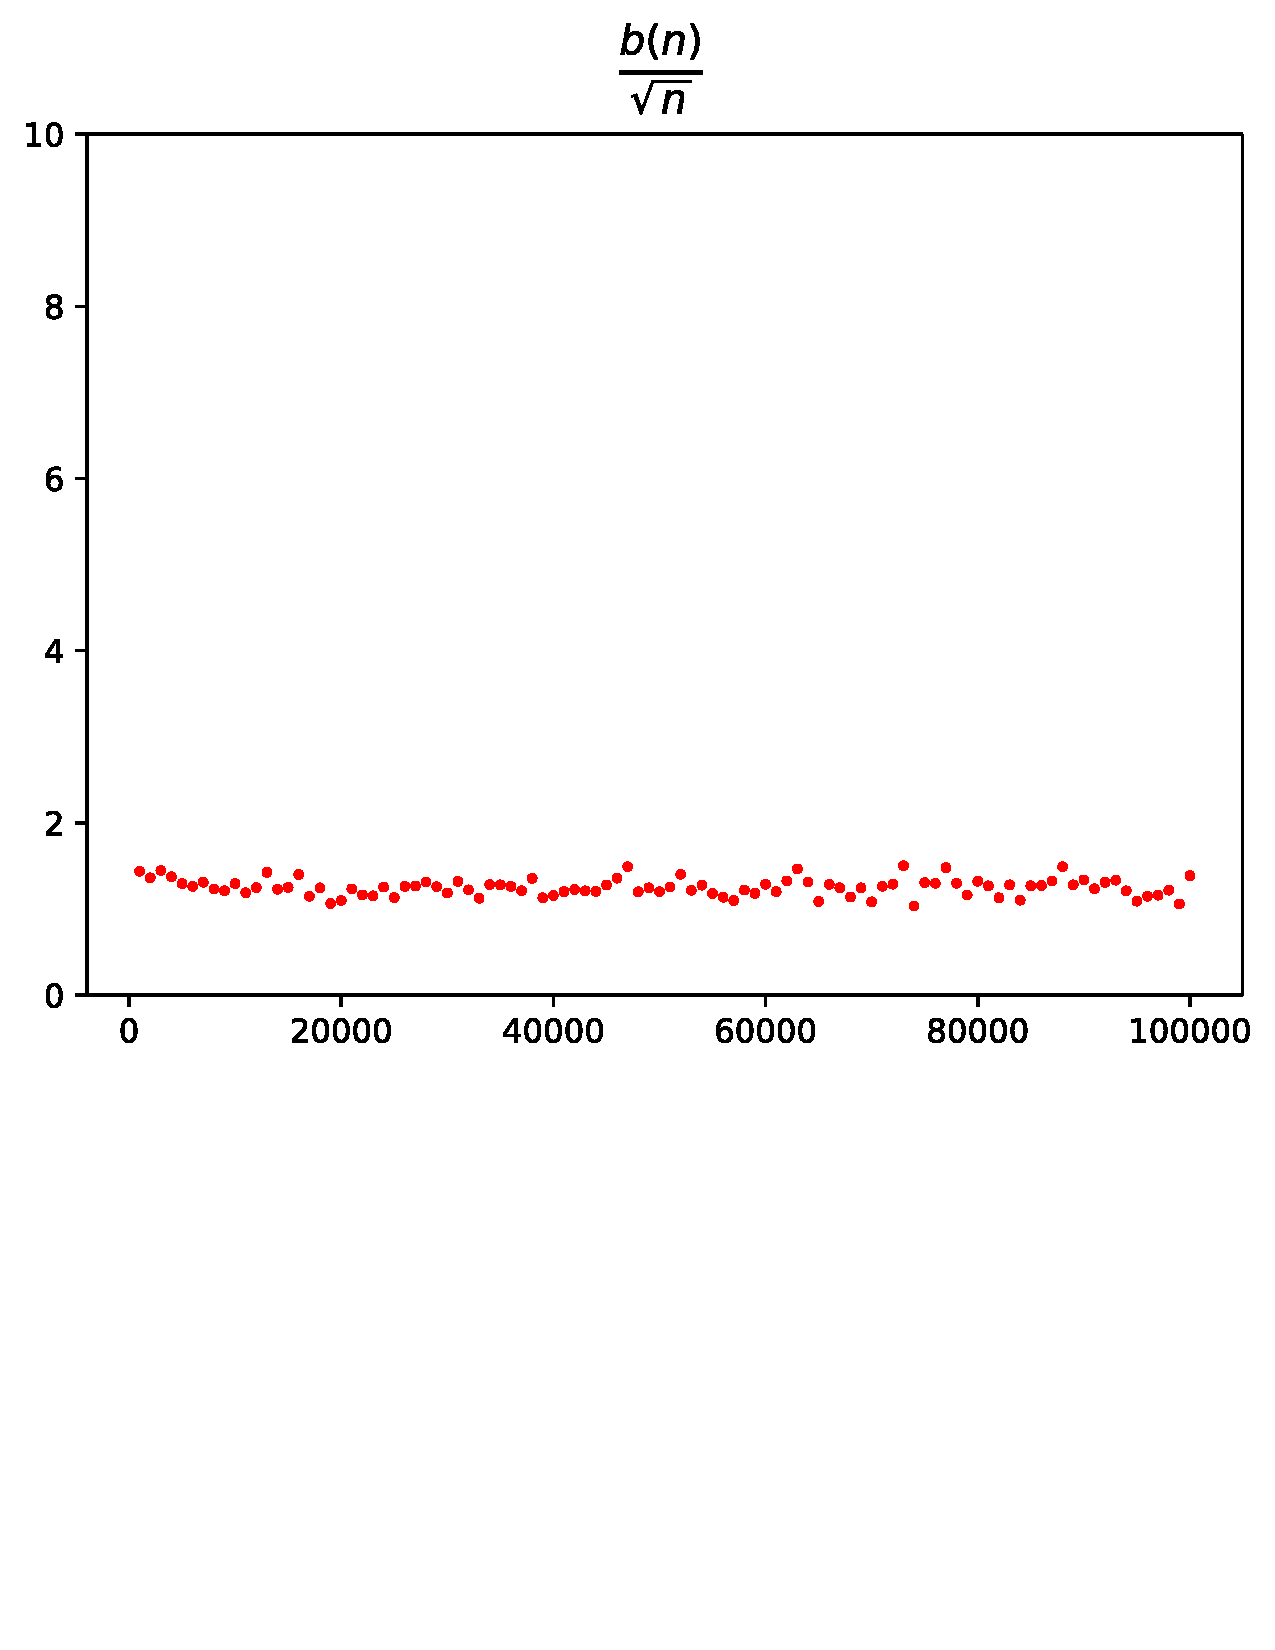
\includegraphics[width=8cm, trim = 0 10cm 0 0, clip]{images/bn2.pdf}
\end{figure}

Chcąc wytłumaczyć nazwę $Birthday$ $paradox$ należy nieco inaczej spojrzeć na przeprowadzony eksperyment. Urny są wtedy dniami roku, a kule ludźmi. Wrzucenie drugiej kuli do tej samej urny po raz pierwszy oznacza, że dwie ososby urodziły się w tym samym dniu roku. Zmienna losowa $B_n$ oznacza średnią liczebność grupy, w której dwie osoby urodziły się tego samego dnia. Okazuje się, że ta liczba jest zaskakująco mała. Dla 365 dni w roku wynosi około 35 (odczytując wartości z wykresów). Stąd $paradox$ w nazwie. \par
$Birthday$ $paradox$ ma znaczenie w przypadku funkcji hashujących, ponieważ oznacza to, że w dużym zbiorze wartości istnieje duże prawdopodobieństwo tego, że dwie różne wartości dadzą taki sam hash. Kryptograficzne funkcje haszujące mają tę własność, że prawdopodobieństwo wygenerowania takich samych hashy dla różnych wartości znaków jest małe, co może uodpornić system na ataki hakerów.

\subsection*{Liczba pustych urn po wrzuceniu $n$ kul}

Na wykresie $U_n$ widać wyraźnie, że wspomniana wielkość zależy liniowo od ilości urn ($n$). Potwierdza to mniejszy wykres, z którego wynika, że $u(n)=\Theta(n)$ Koncentracja wokół wartości średniej jest tutaj bardzo mocna, punkty dla poszczególnych eksperymentów są praktycznie przesłonięte przez wartości średnie. Tutaj wystaczyłoby zbadać tylko $n \leq 20000$.

\begin{figure}[H]
    \centering
    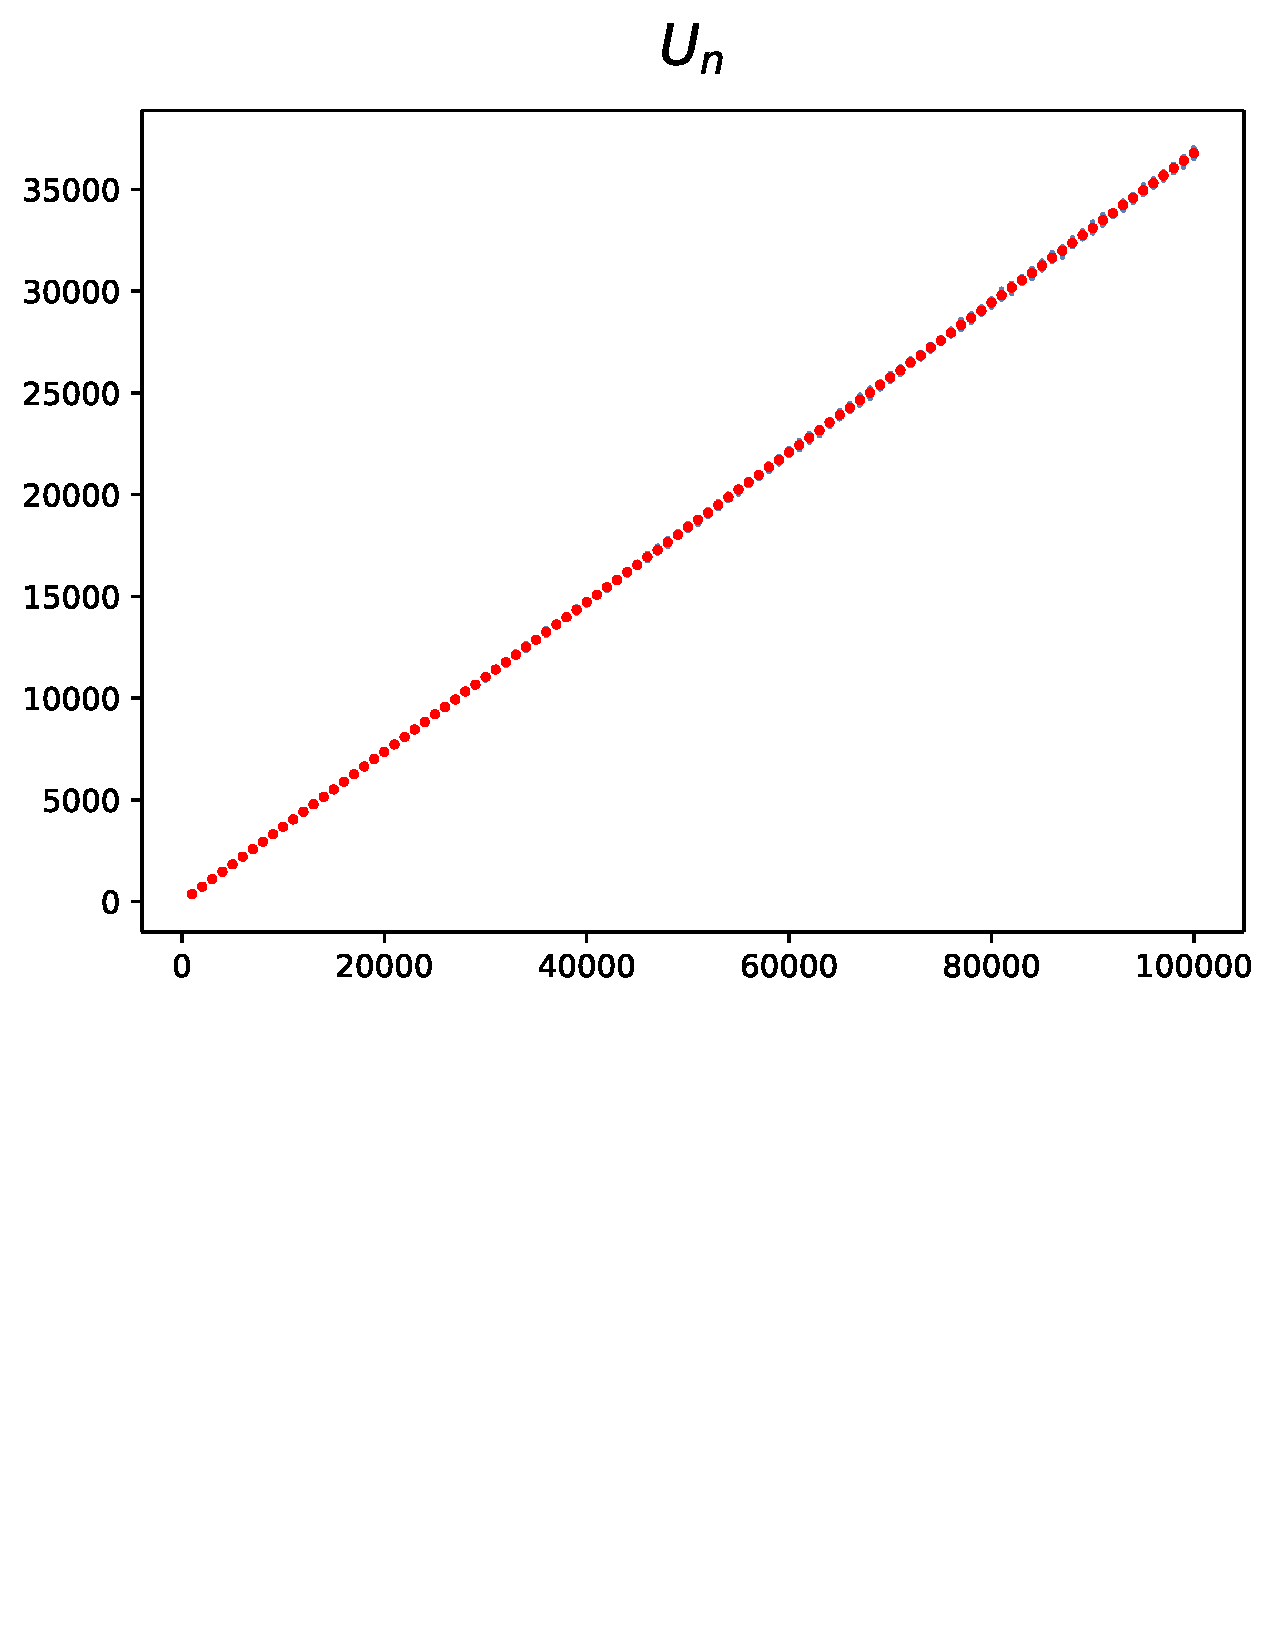
\includegraphics[width=15cm, trim = 0 10cm 0 0, clip]{images/un.pdf}
\end{figure}
\begin{figure}[H]
    \centering
    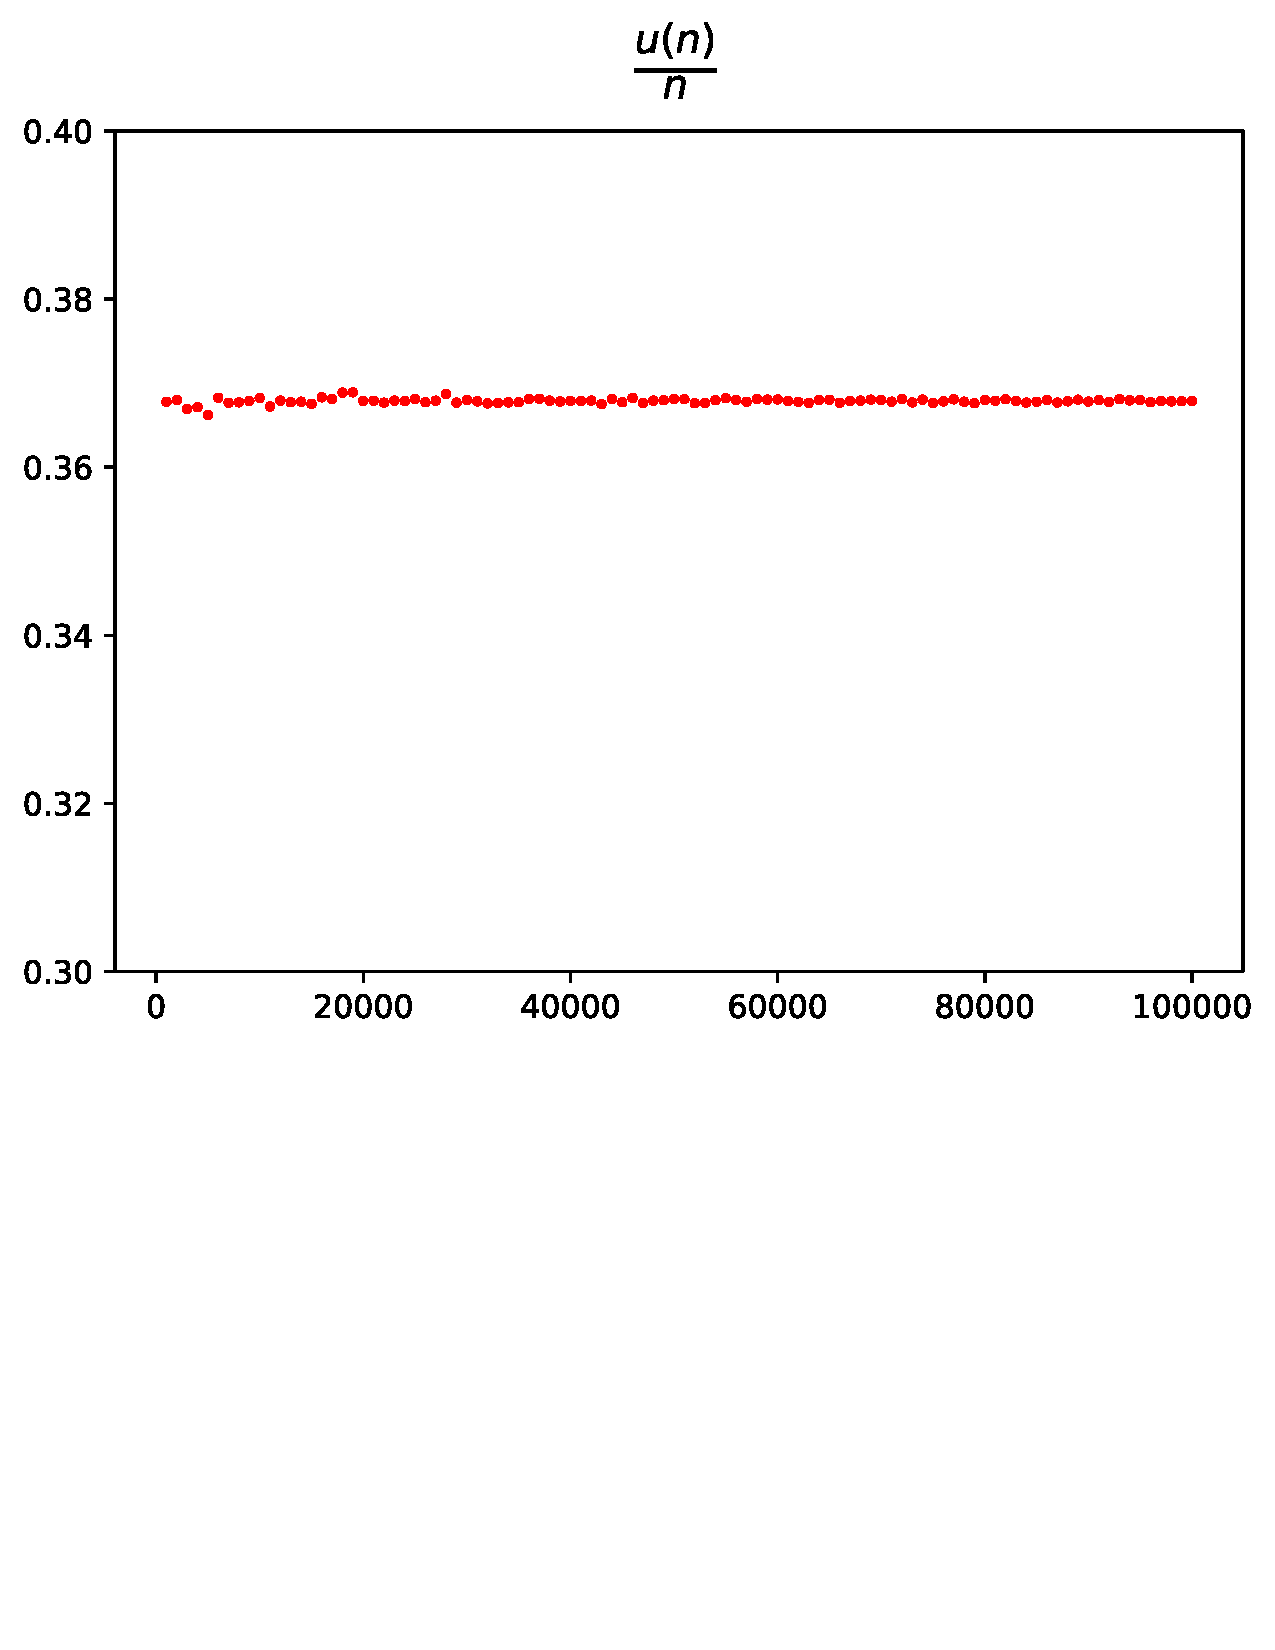
\includegraphics[width=8cm, trim = 0 10cm 0 0, clip]{images/un1.pdf}
\end{figure}

\subsection*{Maksymalna liczba kul w urnie po wrzuceniu $n$ kul}

Punkty dla wartości średnich wielkości $L_n$ na pierwszy rzut oka mogą przypominać funkcję pierwiastka, jednak tempo wzrostu sugeruje, że jest to funkcja logarytmiczna. Sprawdzając jednak tą hipotezę na pierwszym z małych wykresów funkcja ta okazuje się powoli maleć, więc jej wartości mogą zbiegać do 0. Na trzecim z małych wykresów widać, że wartości rosną powoli, ale liniowo. Po analizie dwóch kolejnych uważam, że $l(n)=\Theta(\ln \ln n)$. Na wykresie $L_n$ koncentracja wartości wokół średniej jest duża i nie zmienia się ze wzrostem $n$. Tutaj również można by było zbadać mniejszą liczbę ilości urn, np. $n \leq 60000$.

\begin{figure}[H]
    \centering
    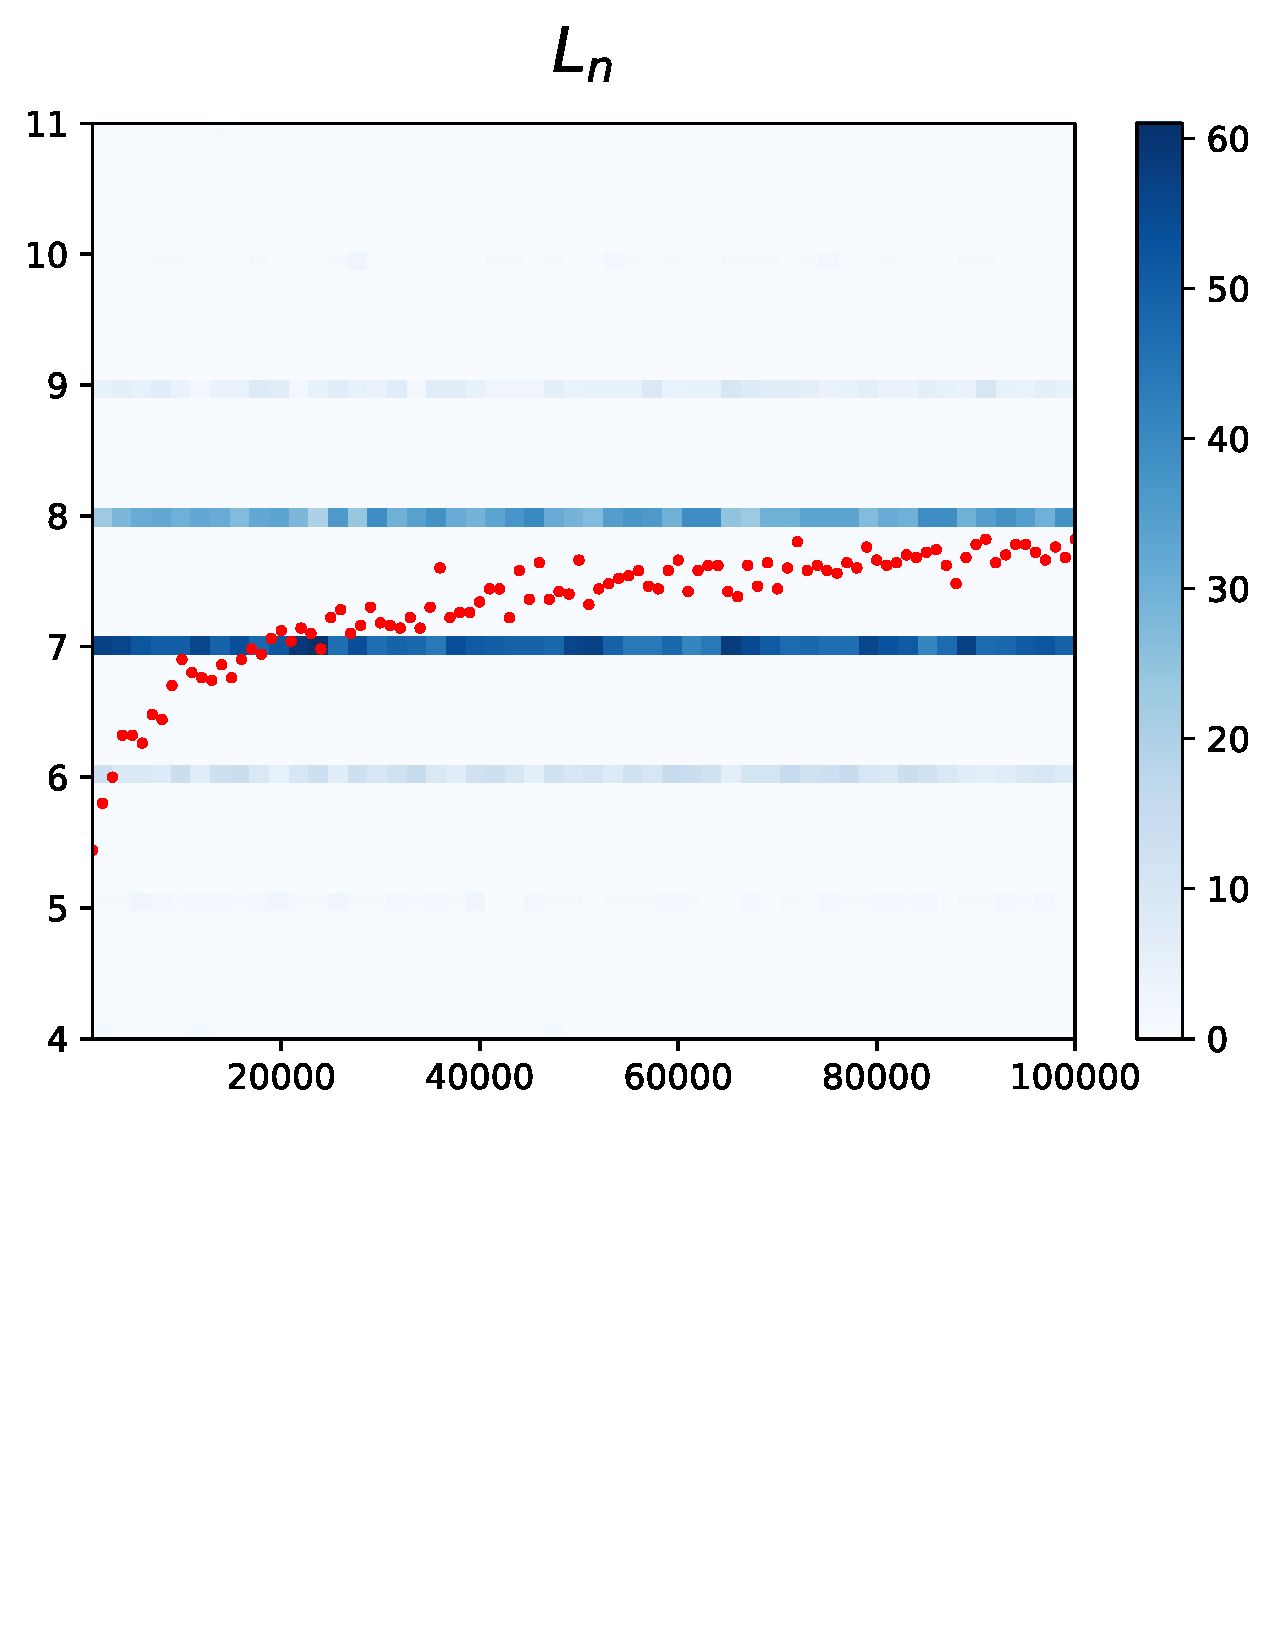
\includegraphics[width=15cm, trim = 0 9cm 0 0, clip]{images/ln.pdf}
\end{figure}
\begin{figure}[H]
    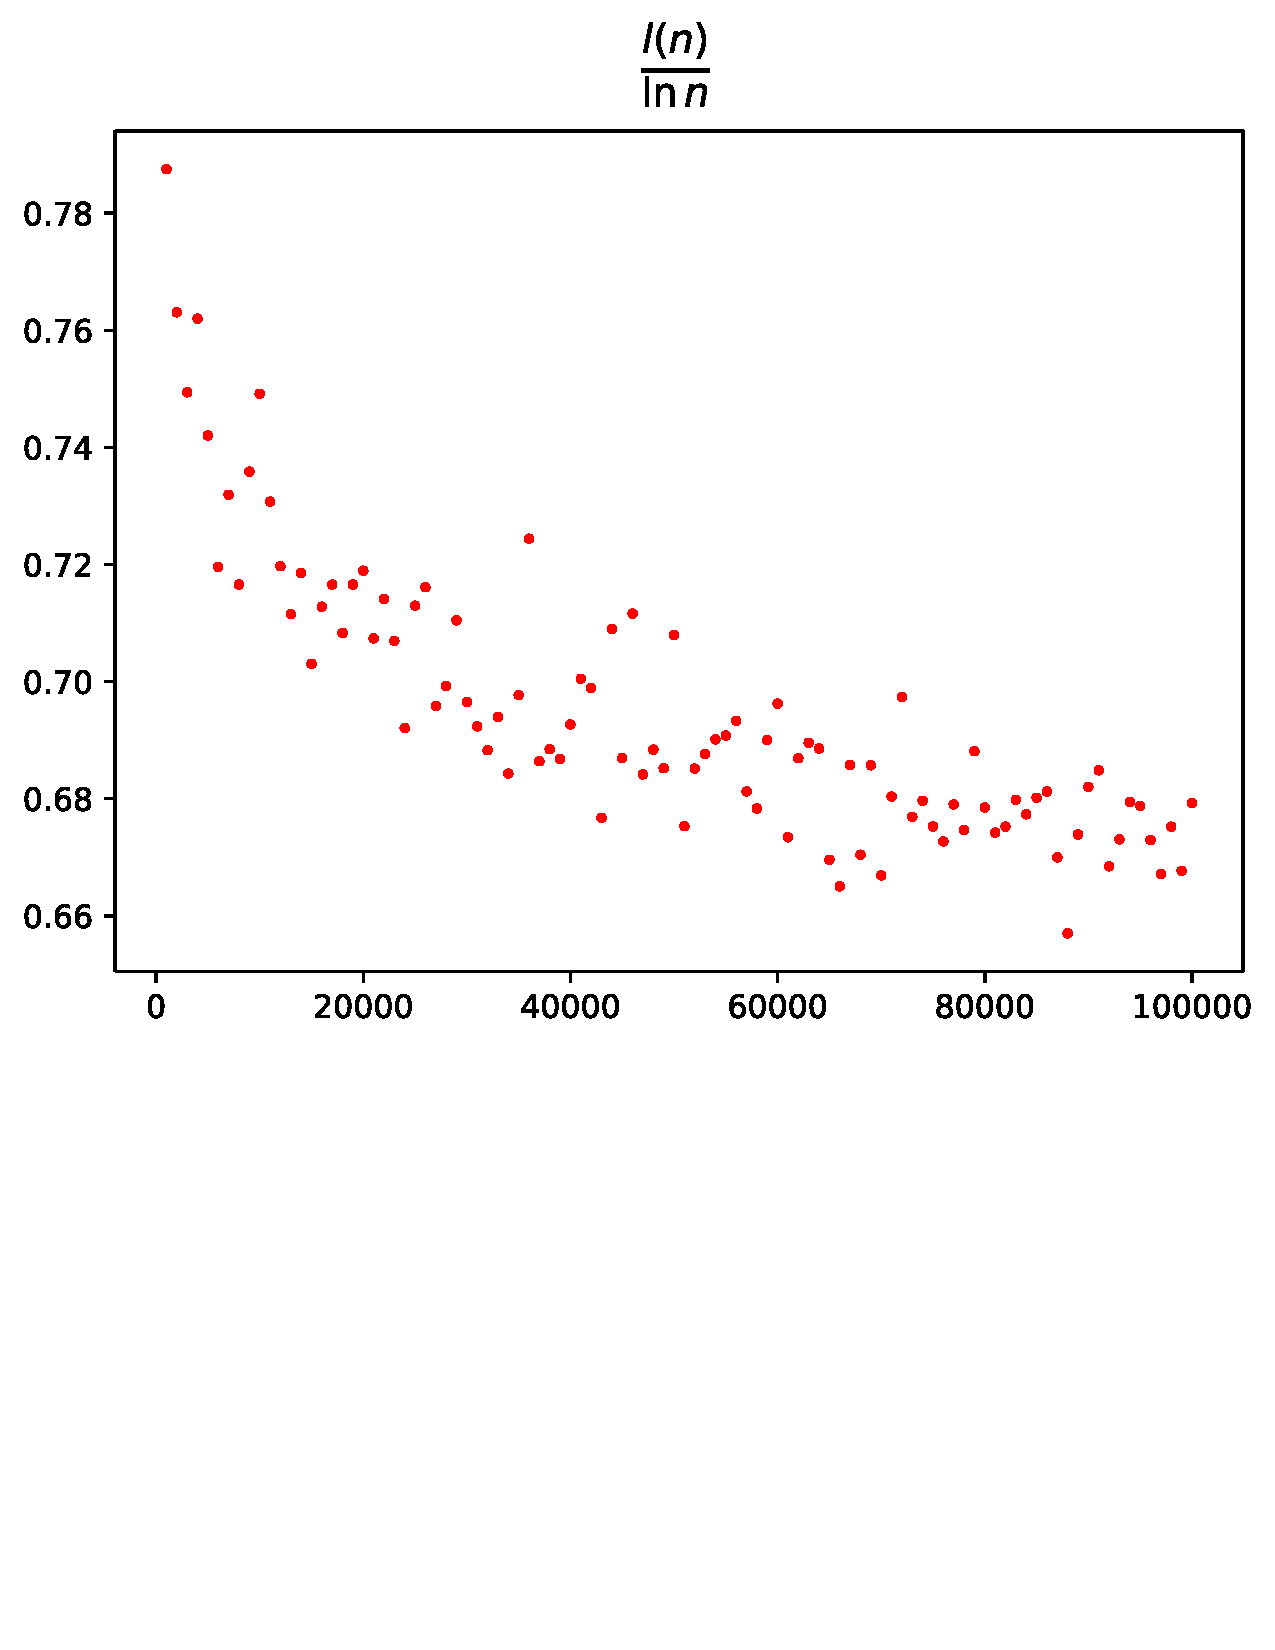
\includegraphics[width=8cm, trim = 0 10cm 0 0, clip]{images/ln1.pdf}
    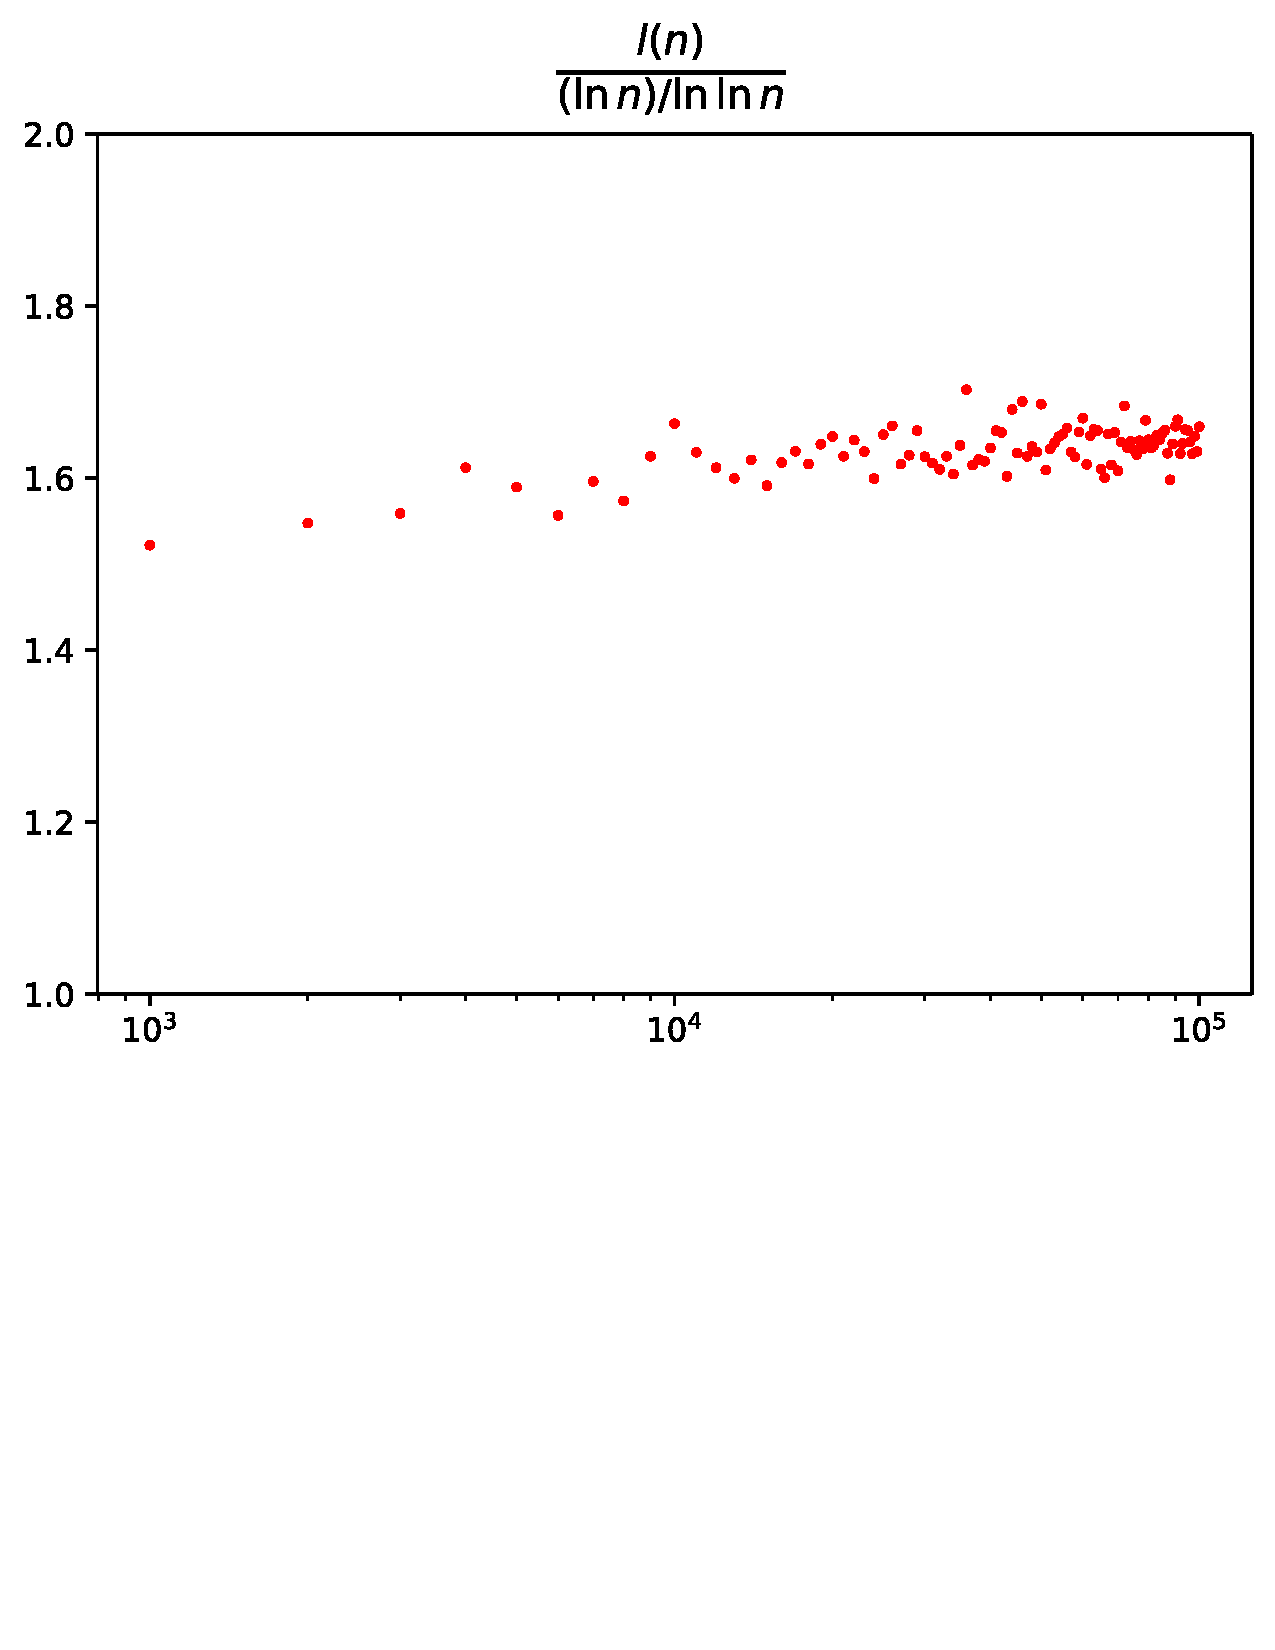
\includegraphics[width=8cm, trim = 0 10cm 0 0, clip]{images/ln2.pdf}
\end{figure}
\begin{figure}[H]
    \centering
    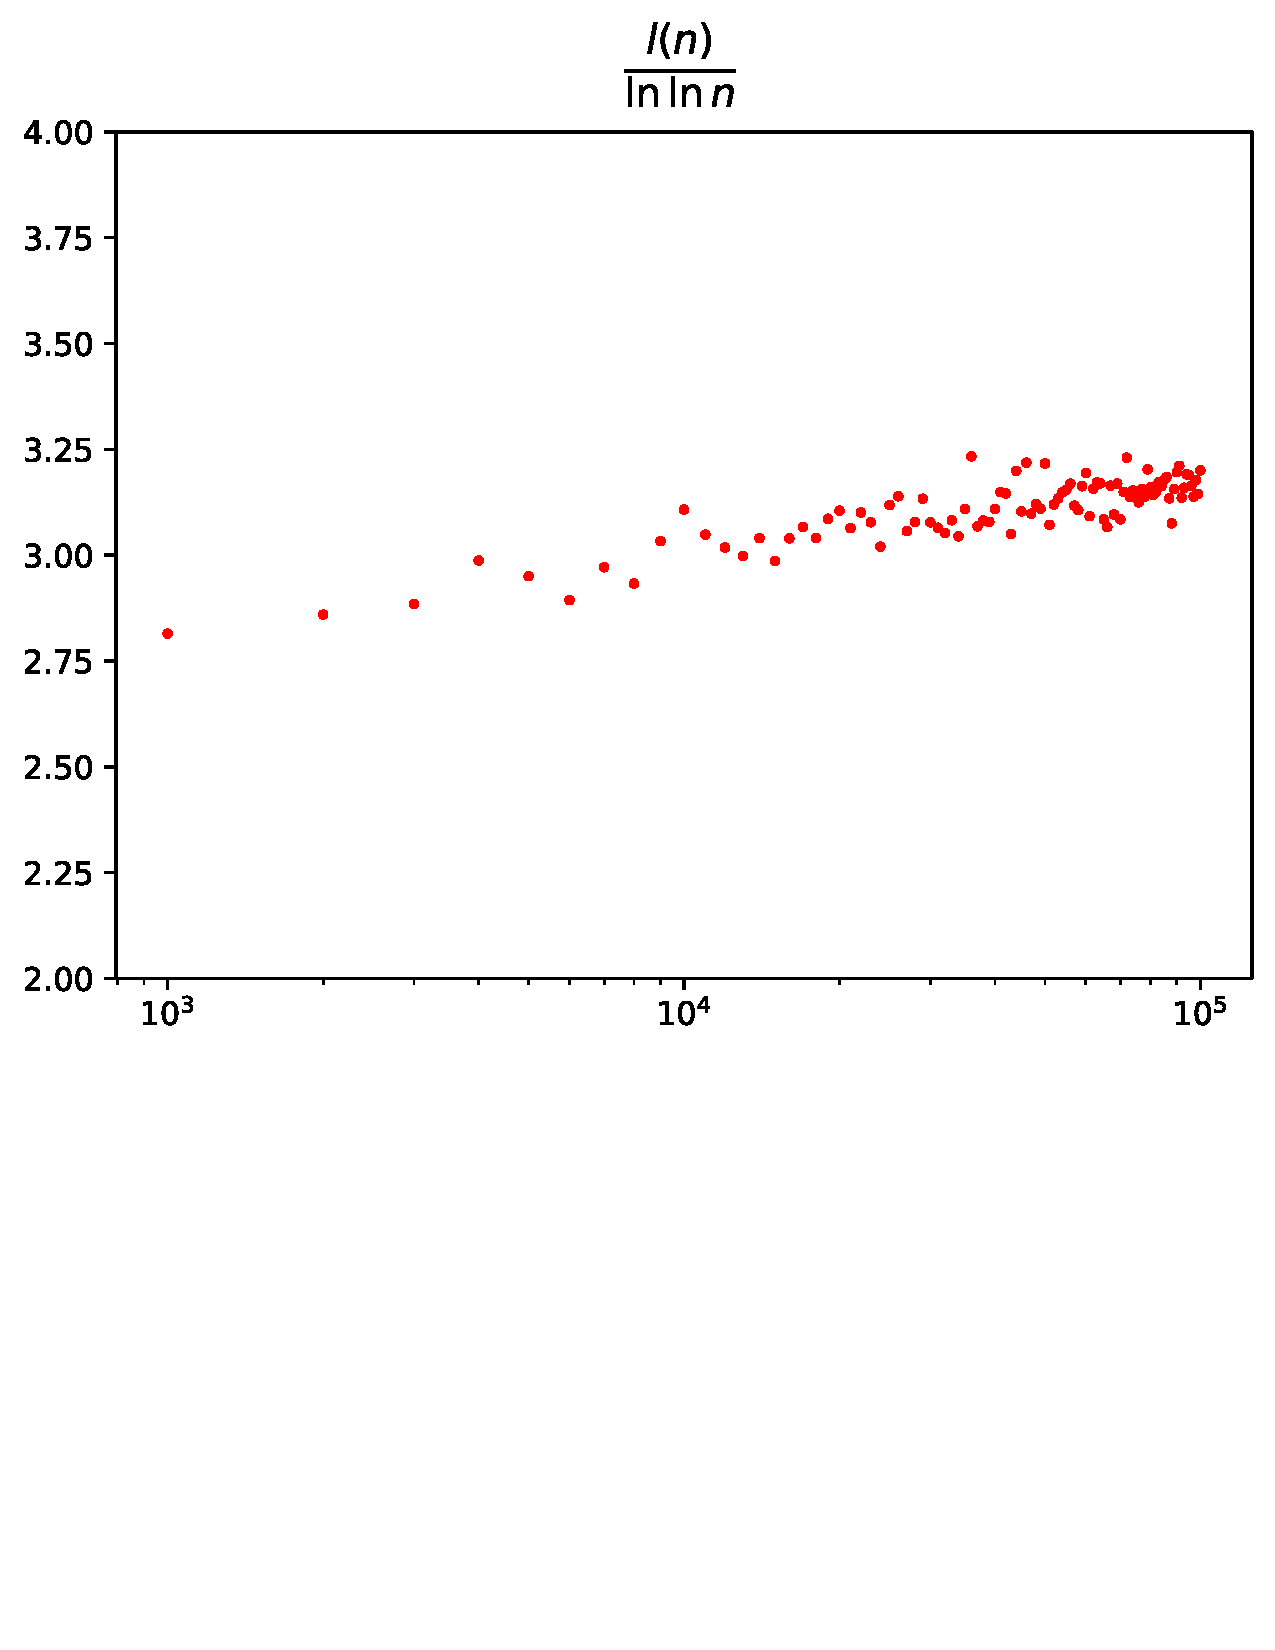
\includegraphics[width=8cm, trim = 0 10cm 0 0, clip]{images/ln3.pdf}
\end{figure}

\subsection*{Minimalna liczba rzutów, po której w każdej z urn jest co najmniej jedna kula}

Wykres wielkości $C_n$ wskazuje, iż ona zależna od funkcji liniowej $n$, jednak po sprawdzeniu tego na pierwszym z małych wykresów wartości wydają się dążyć do nieskończoności. Z drugiego wykresu wynika natomiast, że $c(n)=\Theta(n \cdot \ln n)$. Koncentracja wokół wartości średnich maleje wraz ze wzrostem $n$, jednak jest dość mocna. Trend jest widoczny już dla $n \leq 40000$.

\begin{figure}[H]
    \centering
    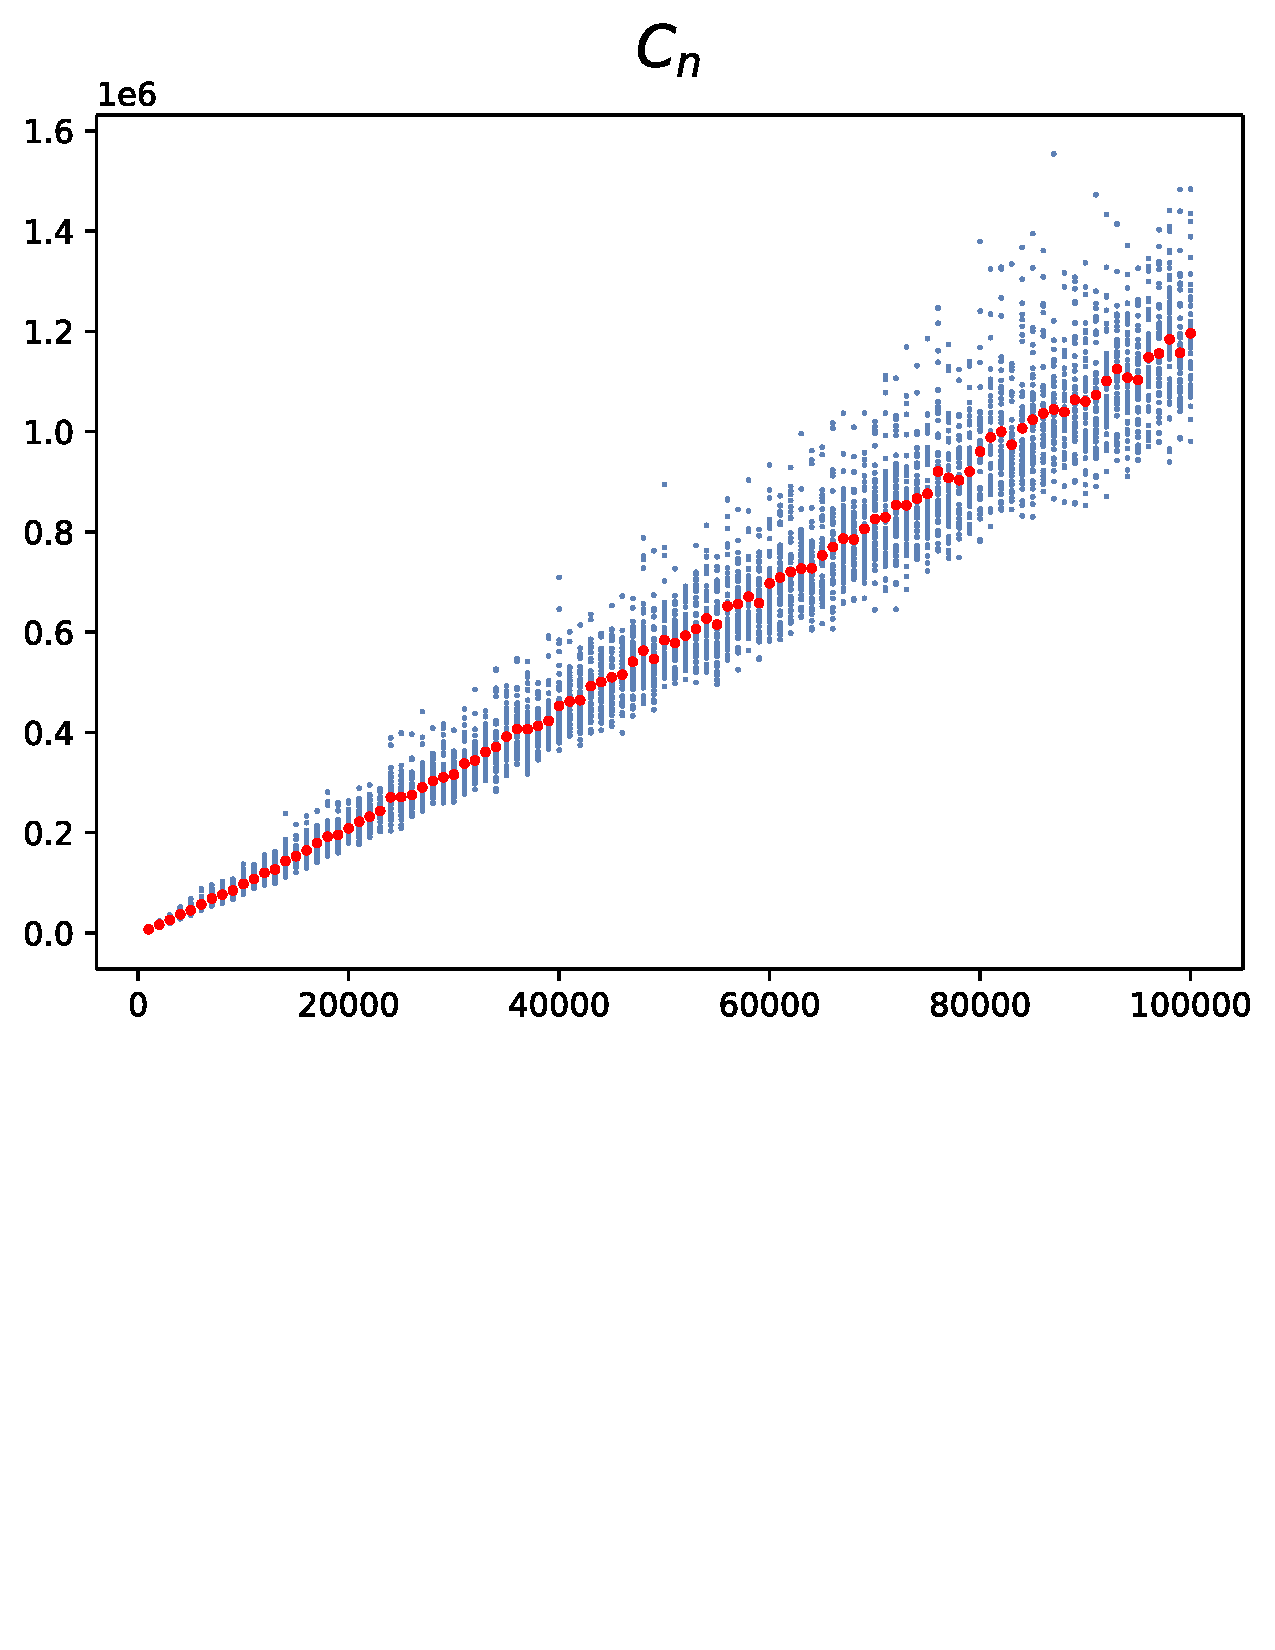
\includegraphics[width=15cm, trim = 0 10cm 0 0, clip]{images/cn.pdf}
\end{figure}
\begin{figure}[H]
    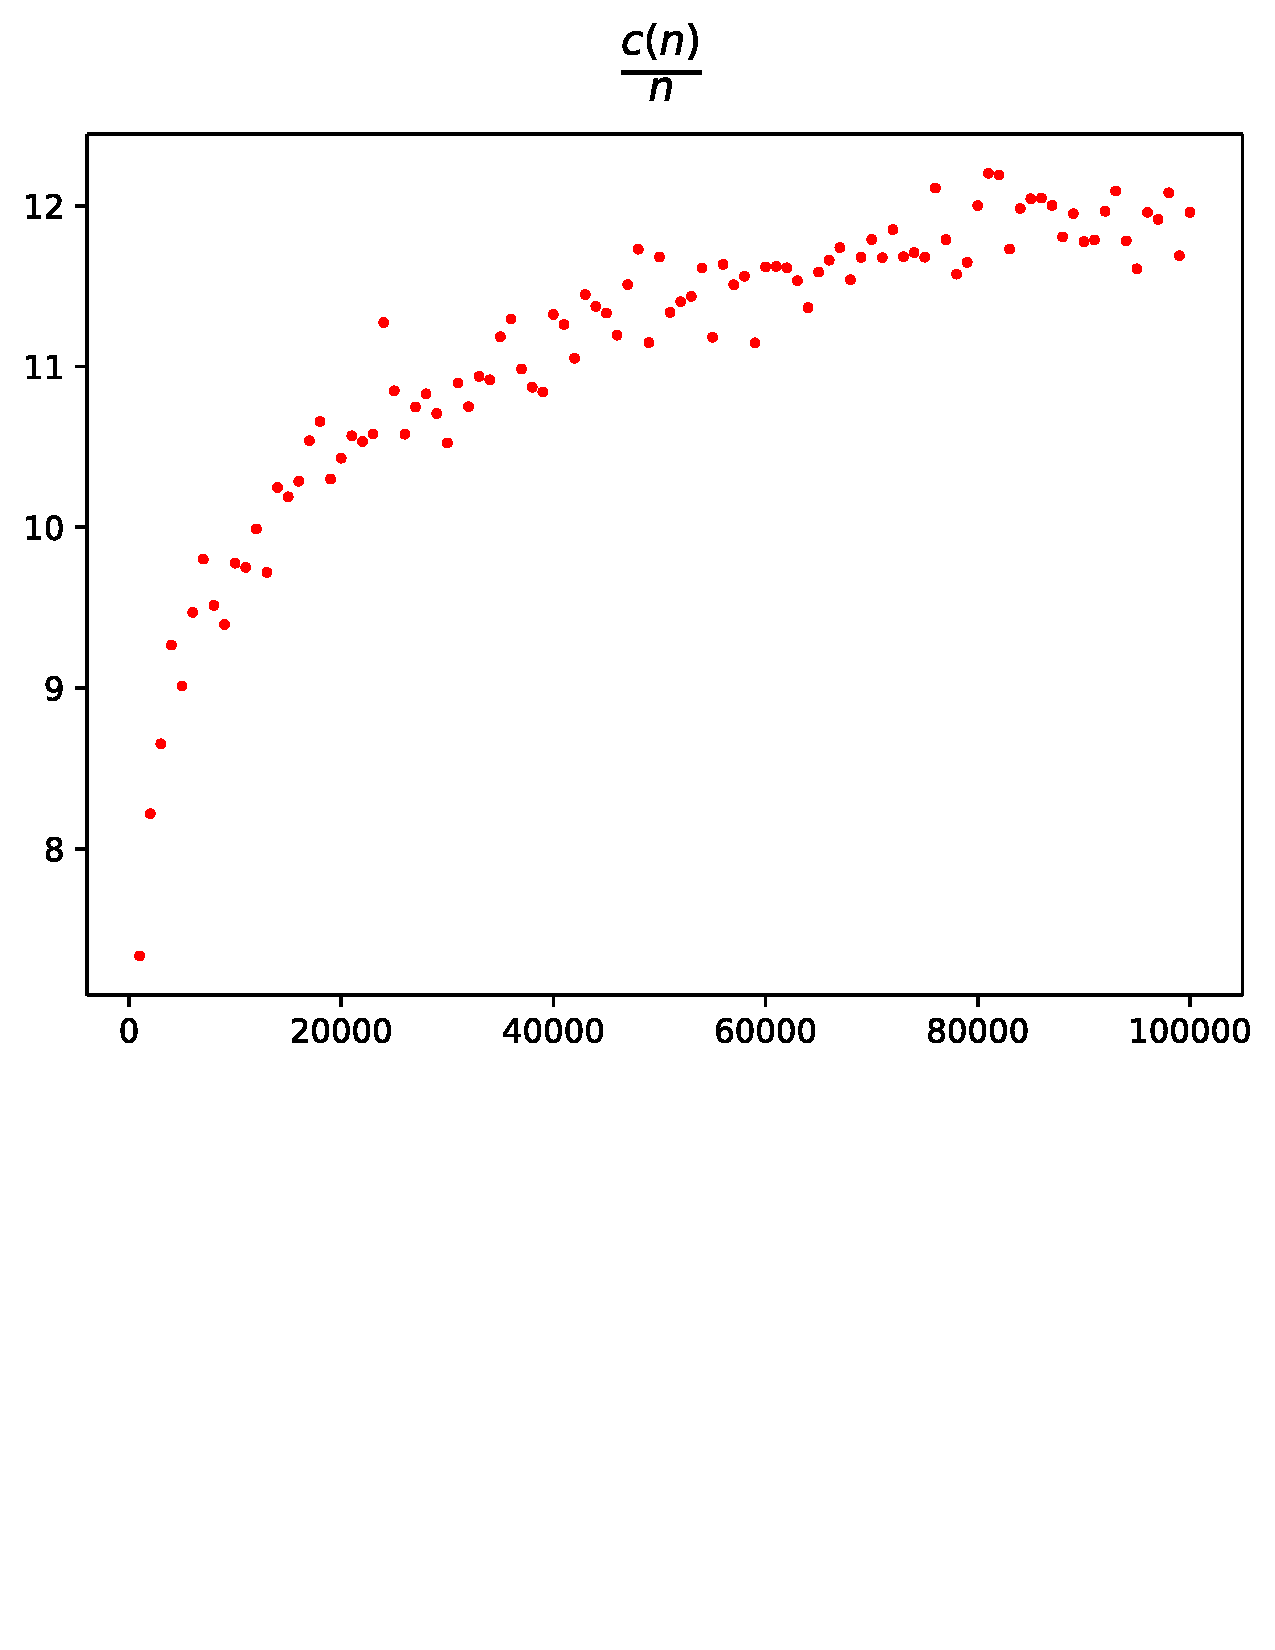
\includegraphics[width=8cm, trim = 0 10cm 0 0, clip]{images/cn1.pdf}
    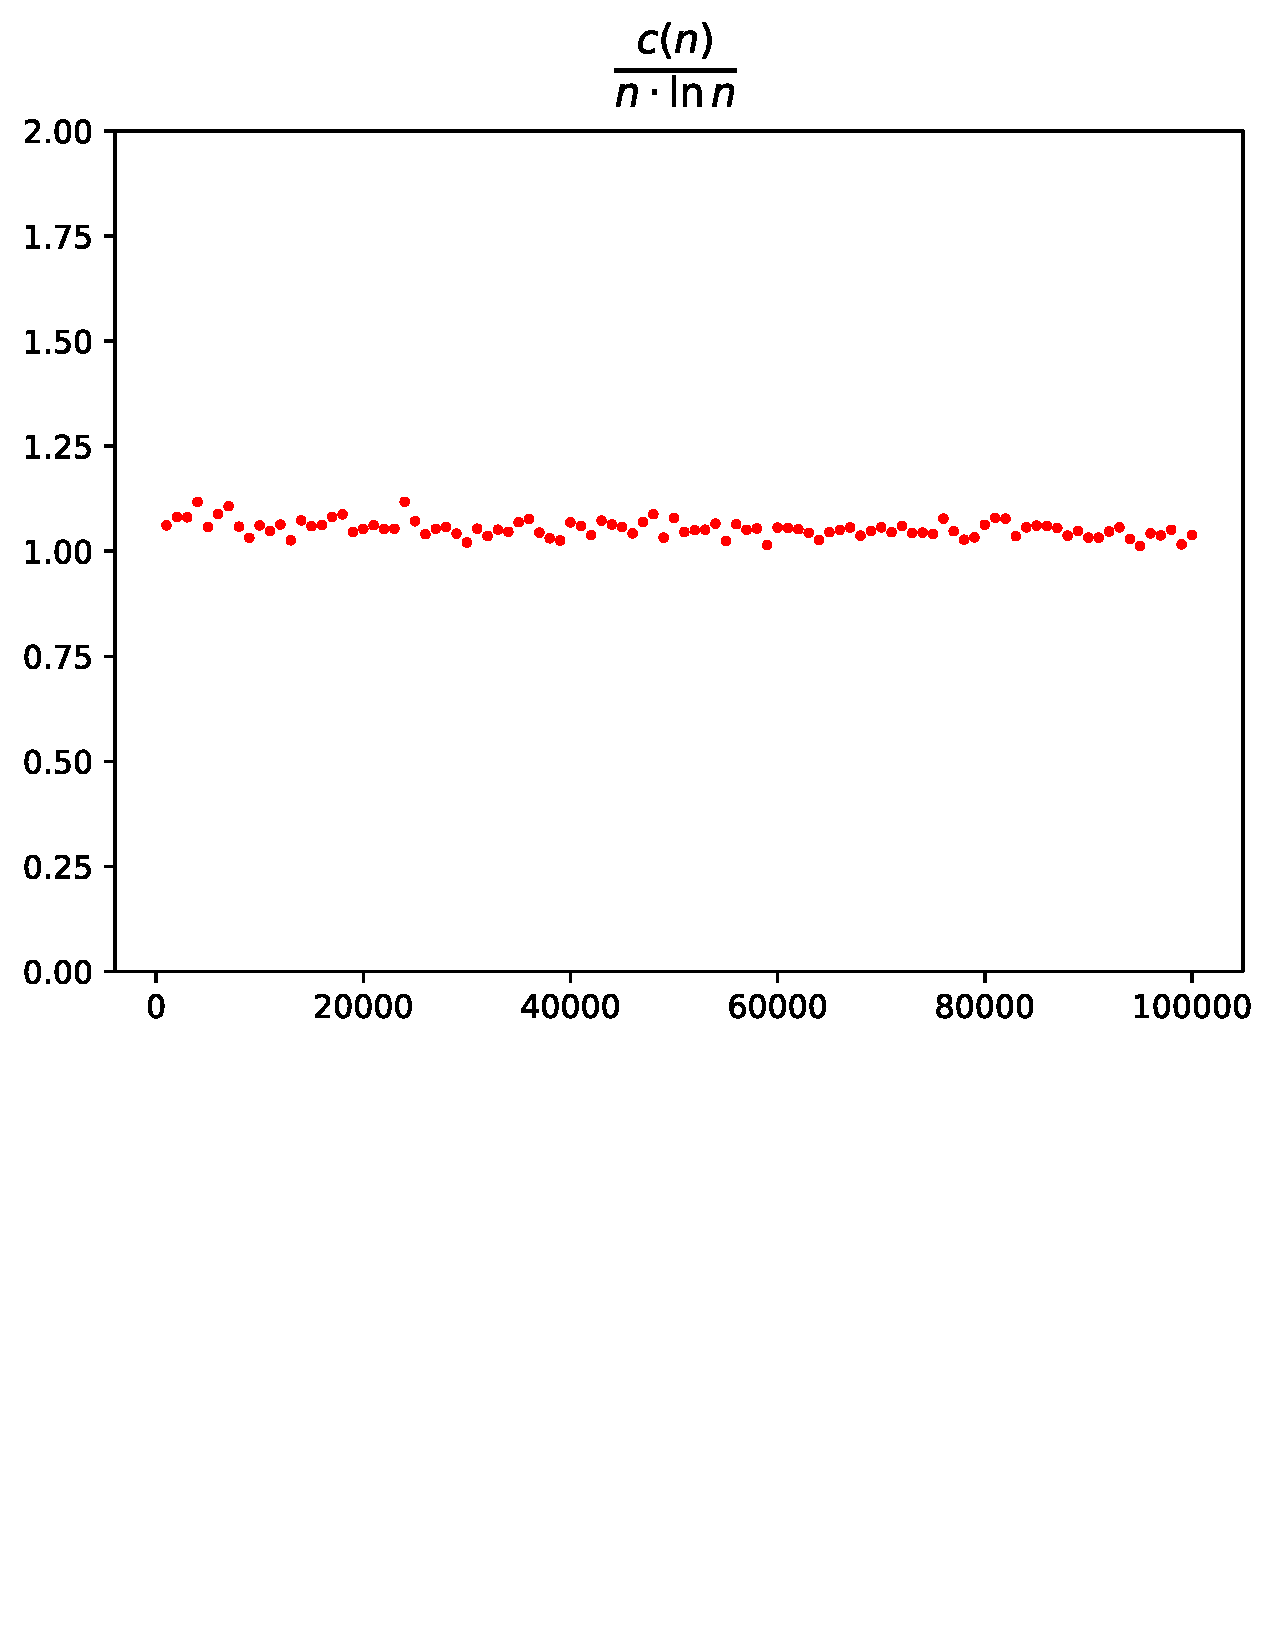
\includegraphics[width=8cm, trim = 0 10cm 0 0, clip]{images/cn2.pdf}
\end{figure}
\begin{figure}[H]
    \centering
    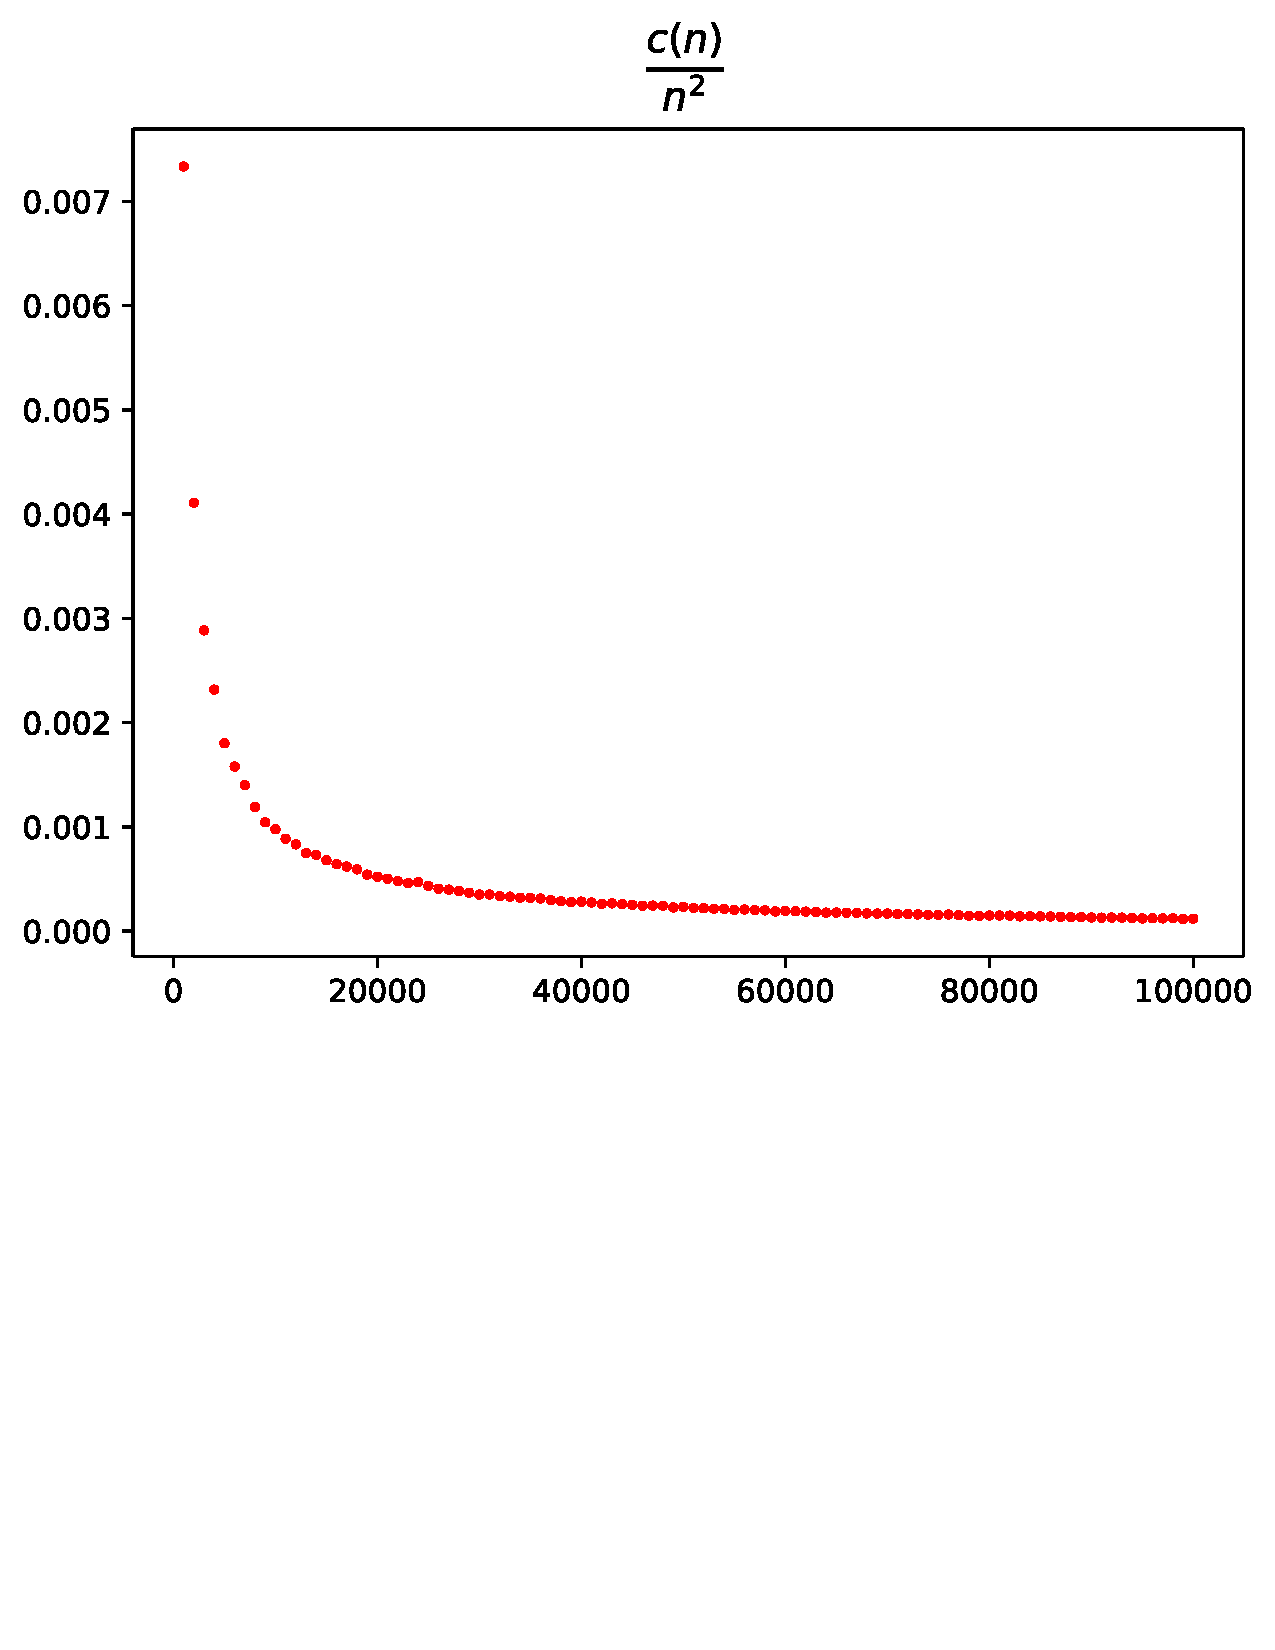
\includegraphics[width=8cm, trim = 0 10cm 0 0, clip]{images/cn3.pdf}
\end{figure}

Nawiązując do nazwy $Coupon$ $collector$ $problem$ można inaczej opisać przeprowadzony eksperyment. Urny są uczestnikami gry, która kończy się, gdy wszyscy uczestnicy znajdą co najmniej jeden kupon (o ile znalezienie kuponu przez każdego uczestnika jest równie prawdopodobne), czyli w naszej sytuacji, gdy kula zostanie wrzucona do urny. Zmienna losowa $C_n$ opisuje wtedy średnią liczbę poukrywanych kuponów, dla której każdy gracz będzie miał co najmniej jeden, czyli gra się zakończy.

\subsection*{Minimalna liczba rzutów, po której w każdej z urn są co najmniej dwie kule}

Wykres $D_n$ bardzo przypomina wykres $C_n$ i podobnie z mniejszych wykresów wynika, że $d(n)=\Theta(n \cdot \ln n)$. Koncentracja wokół wartości średnich jest widoczna i maleje wraz ze wzrostem $n$. Trend jest widoczny już dla $n \leq 40000$.

\begin{figure}[H]
    \centering
    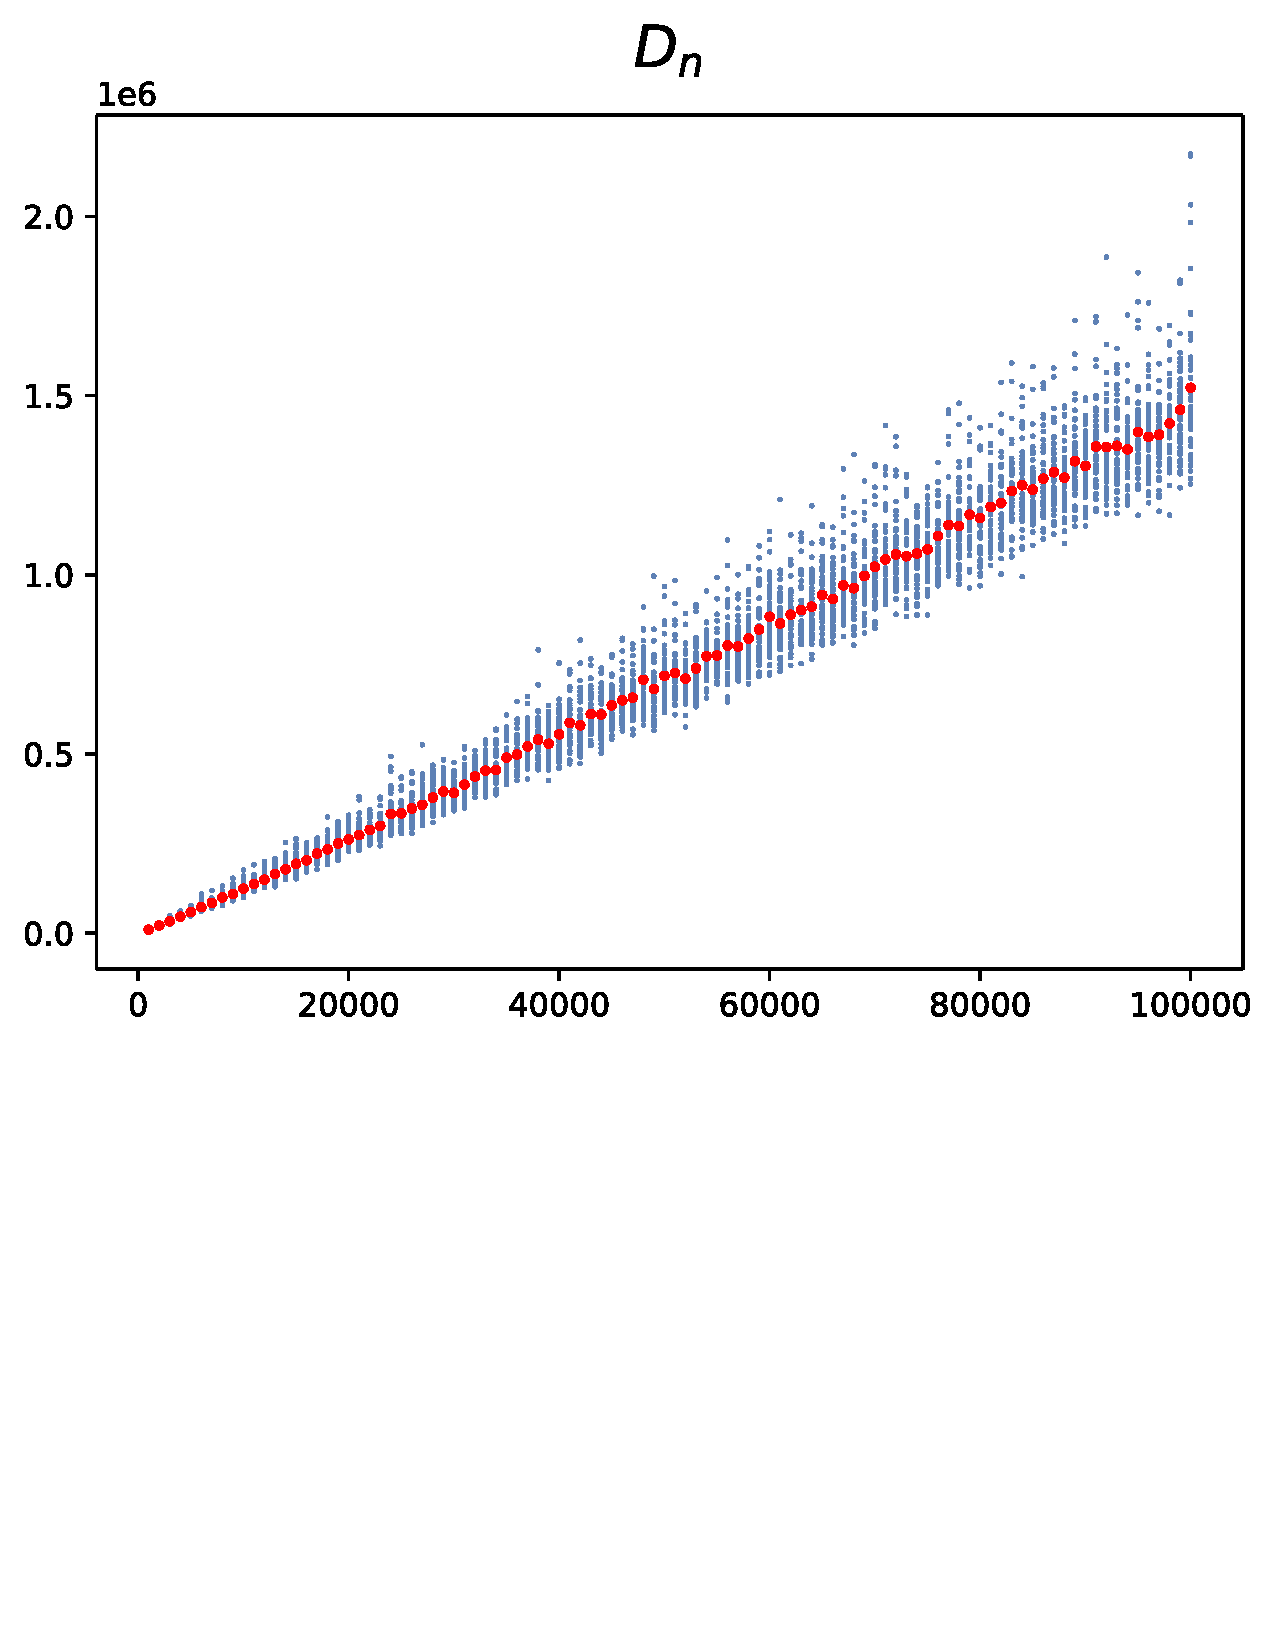
\includegraphics[width=15cm, trim = 0 10cm 0 0, clip]{images/dn.pdf}
\end{figure}
\begin{figure}[H]
    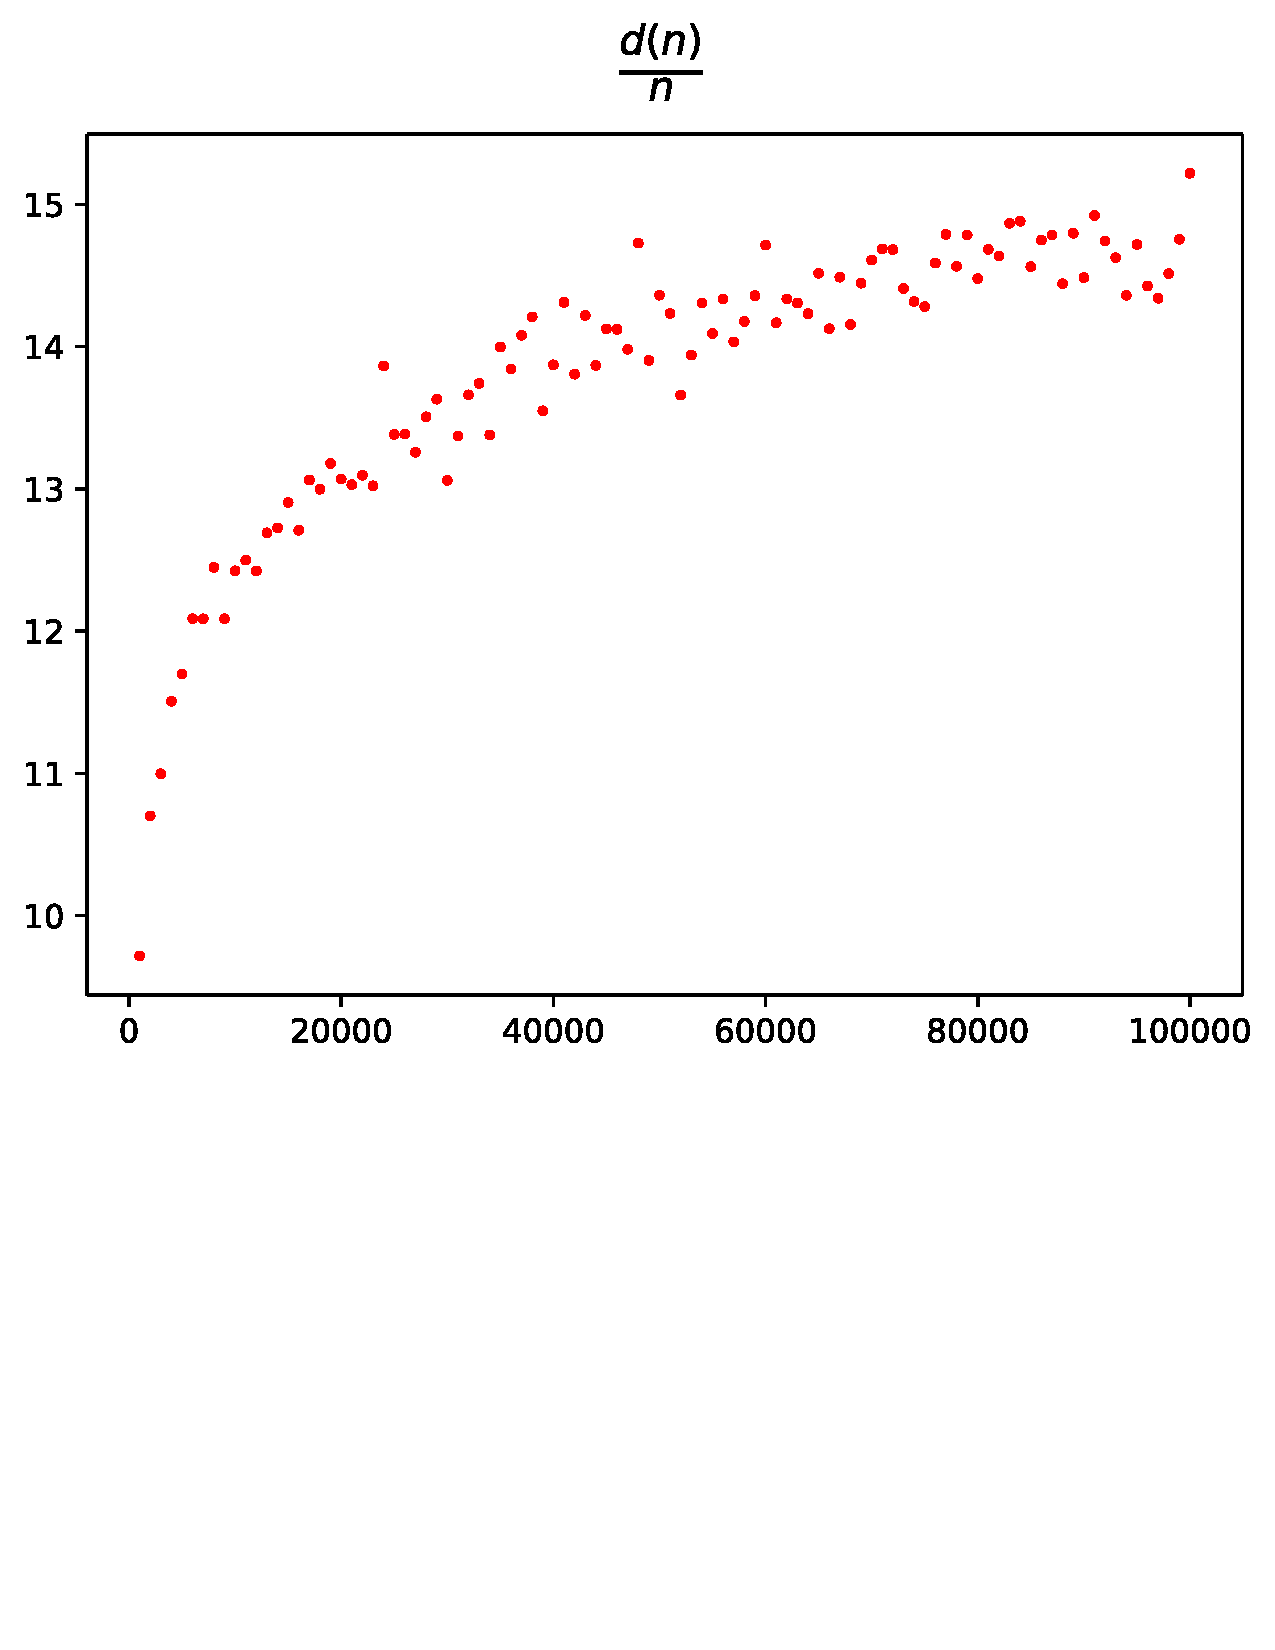
\includegraphics[width=8cm, trim = 0 10cm 0 0, clip]{images/dn1.pdf}
    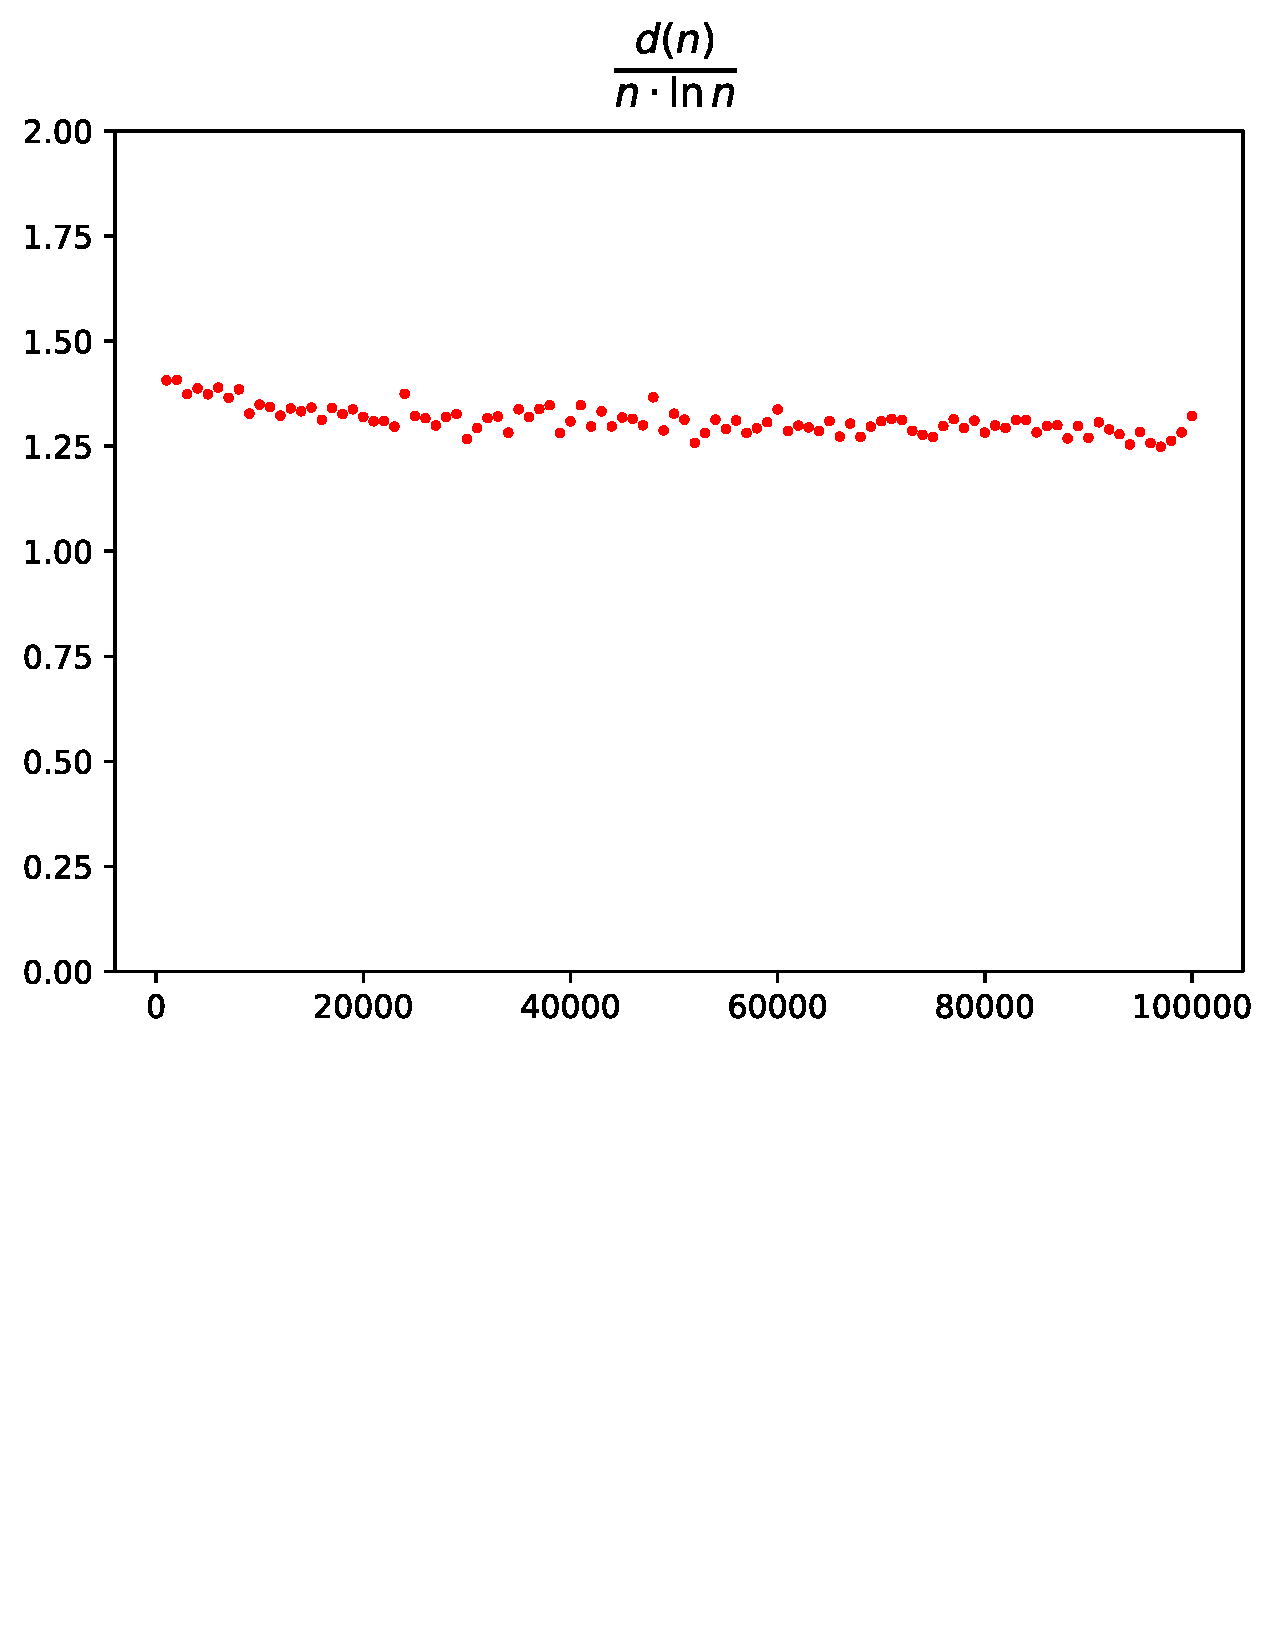
\includegraphics[width=8cm, trim = 0 10cm 0 0, clip]{images/dn2.pdf}
\end{figure}
\begin{figure}[H]
    \centering
    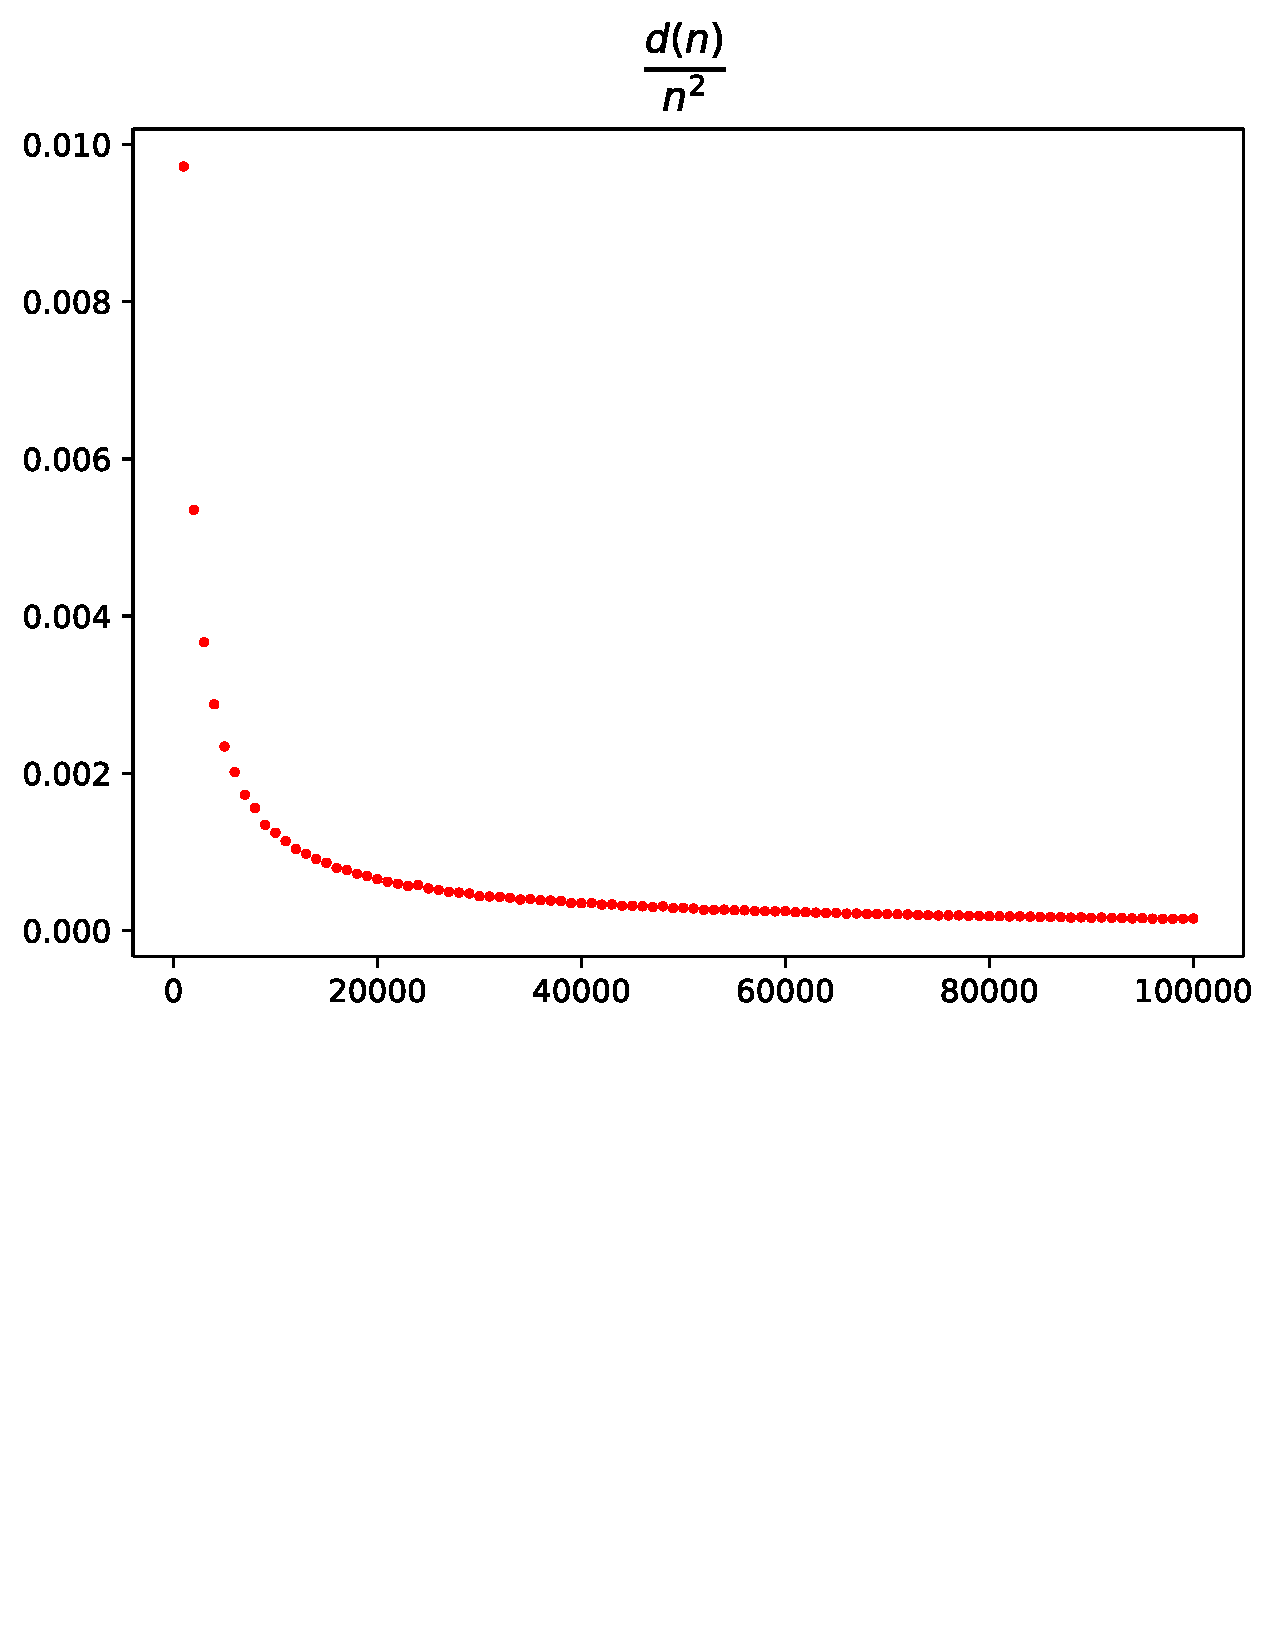
\includegraphics[width=8cm, trim = 0 10cm 0 0, clip]{images/dn3.pdf}
\end{figure}

\subsection*{Minimalna liczba rzutów od momentu $C_n$ do $D_n$}

Różnica $D_n - C_n$ rośnie zdecydowanie wolniej niż $C_n$ i $D_n$. Tutaj na mniejszych wykresach widać, że badana wielkość nie jest liniowa, ponieważ wartości na pierwszym wykresie rosną wraz ze wzrostem $n$. Na drugim z małych wykresów widać, że wartości maleją, natomiast na trzecim są równo skoncentrowane wokół ich wartości średniej. Stąd stawiam hipotezę, że $d(n) - c(n) = \Theta(n \cdot \ln \ln n)$. Koncentracja wokół wartości średnich maleje wraz ze wzrostem $n$ i ponownie trend jest dobrze widoczny już dla $n \leq 40000$.

\begin{figure}[H]
    \centering
    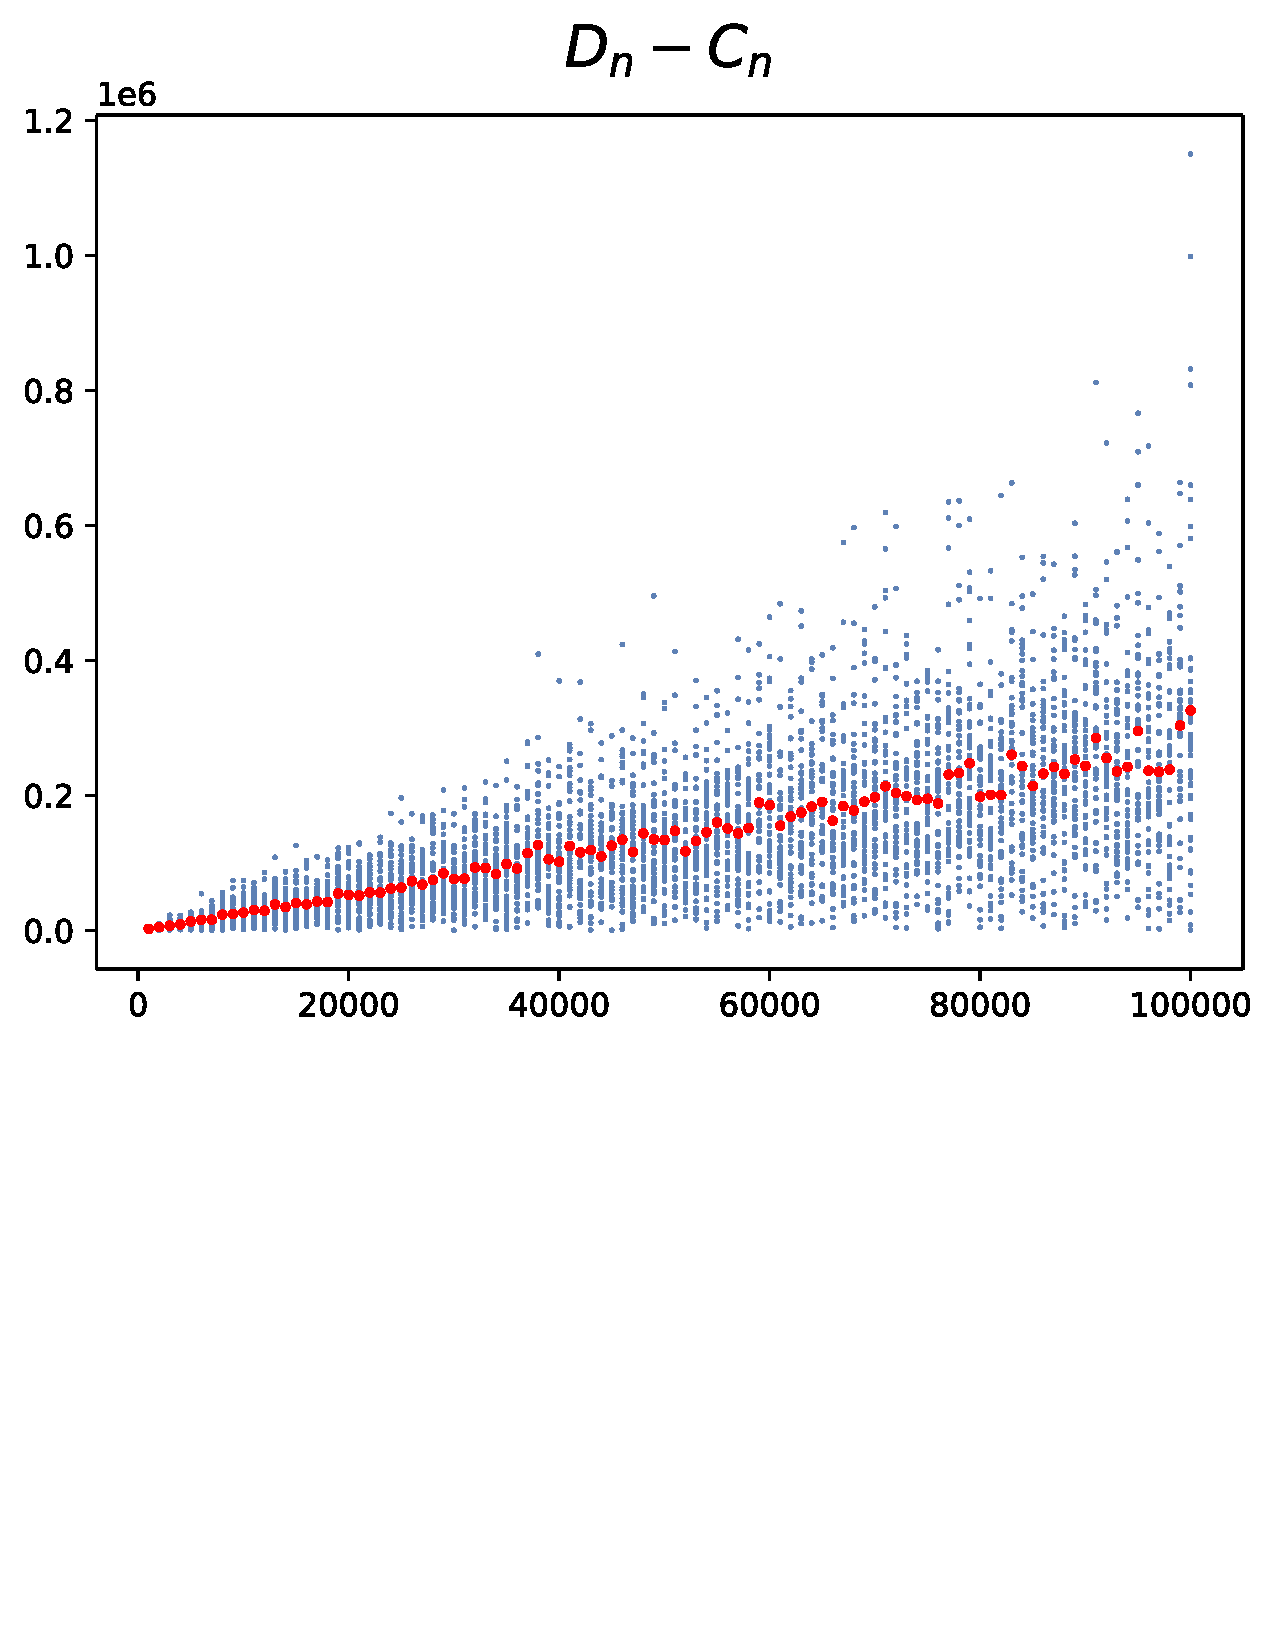
\includegraphics[width=15cm, trim = 0 10cm 0 0, clip]{images/dn-cn.pdf}
\end{figure}
\begin{figure}[H]
    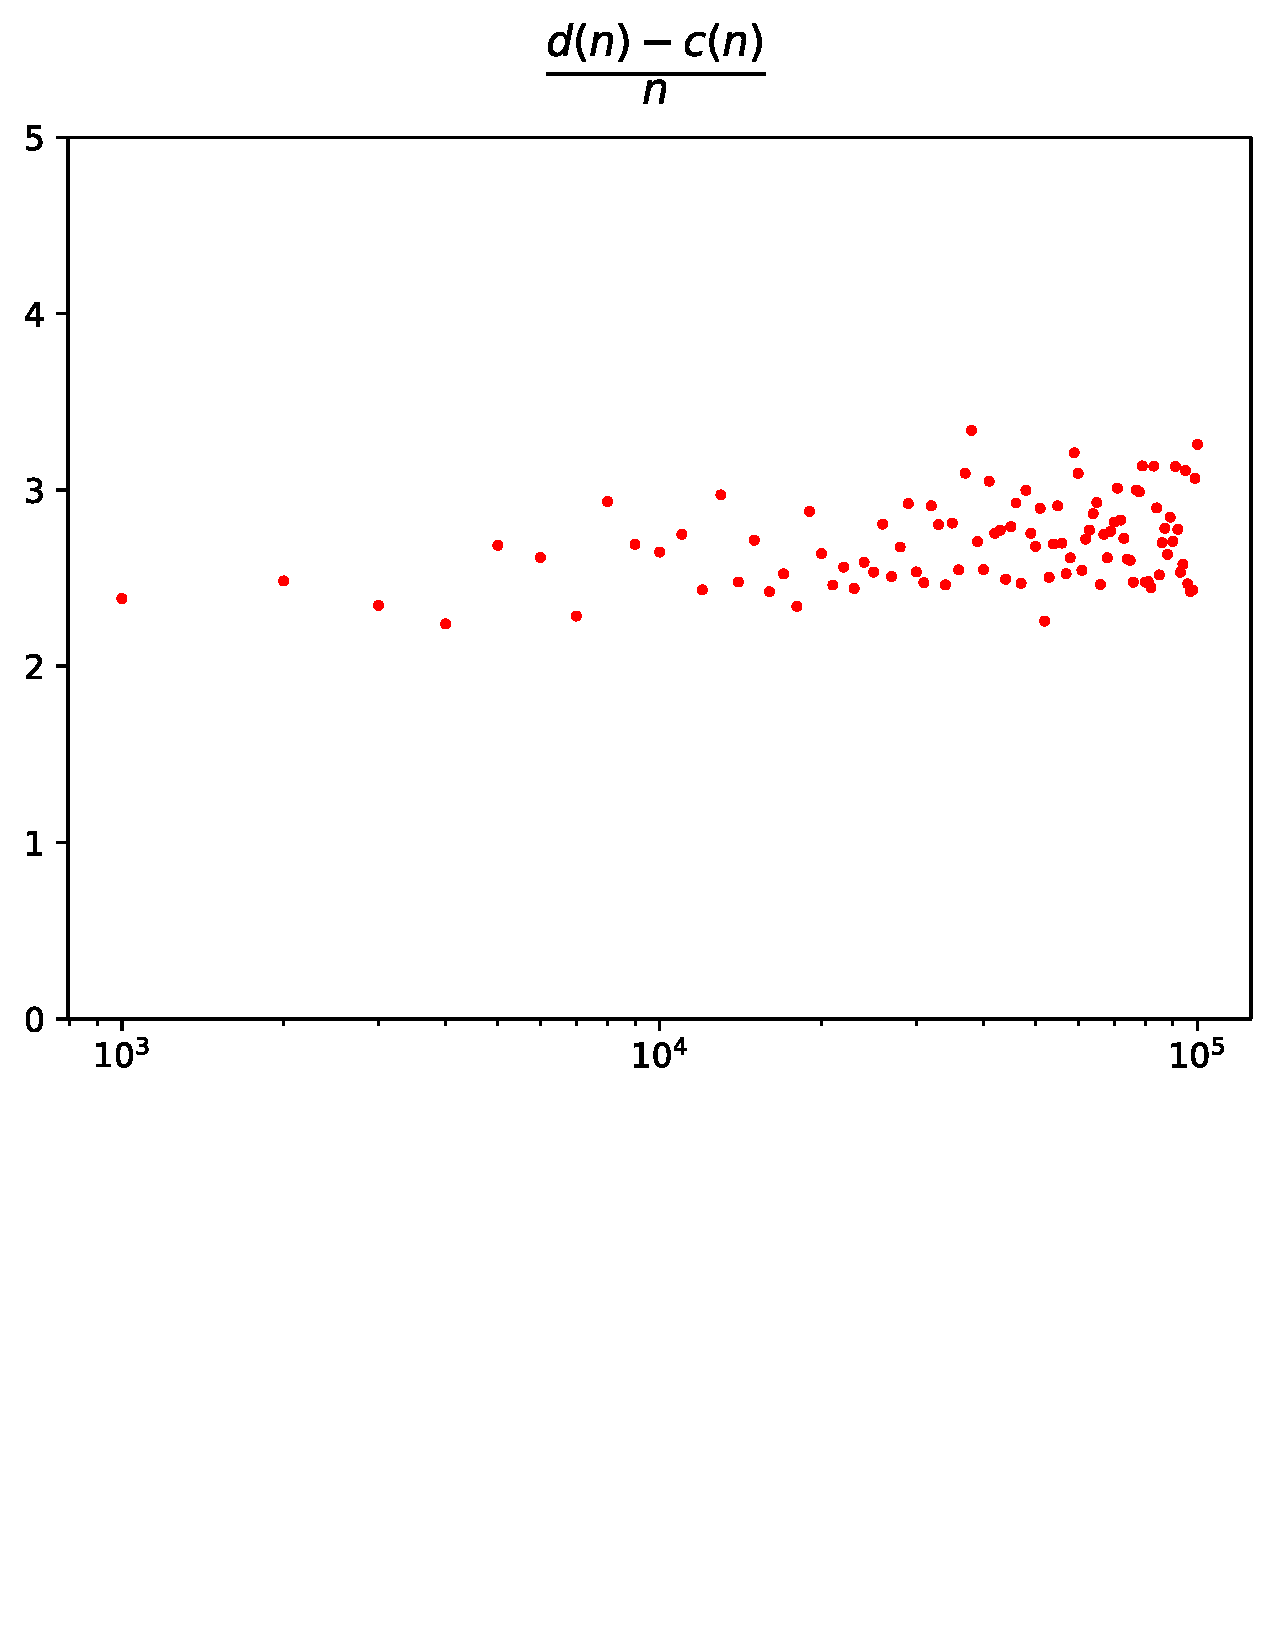
\includegraphics[width=8cm, trim = 0 9cm 0 0, clip]{images/dn-cn1.pdf}
    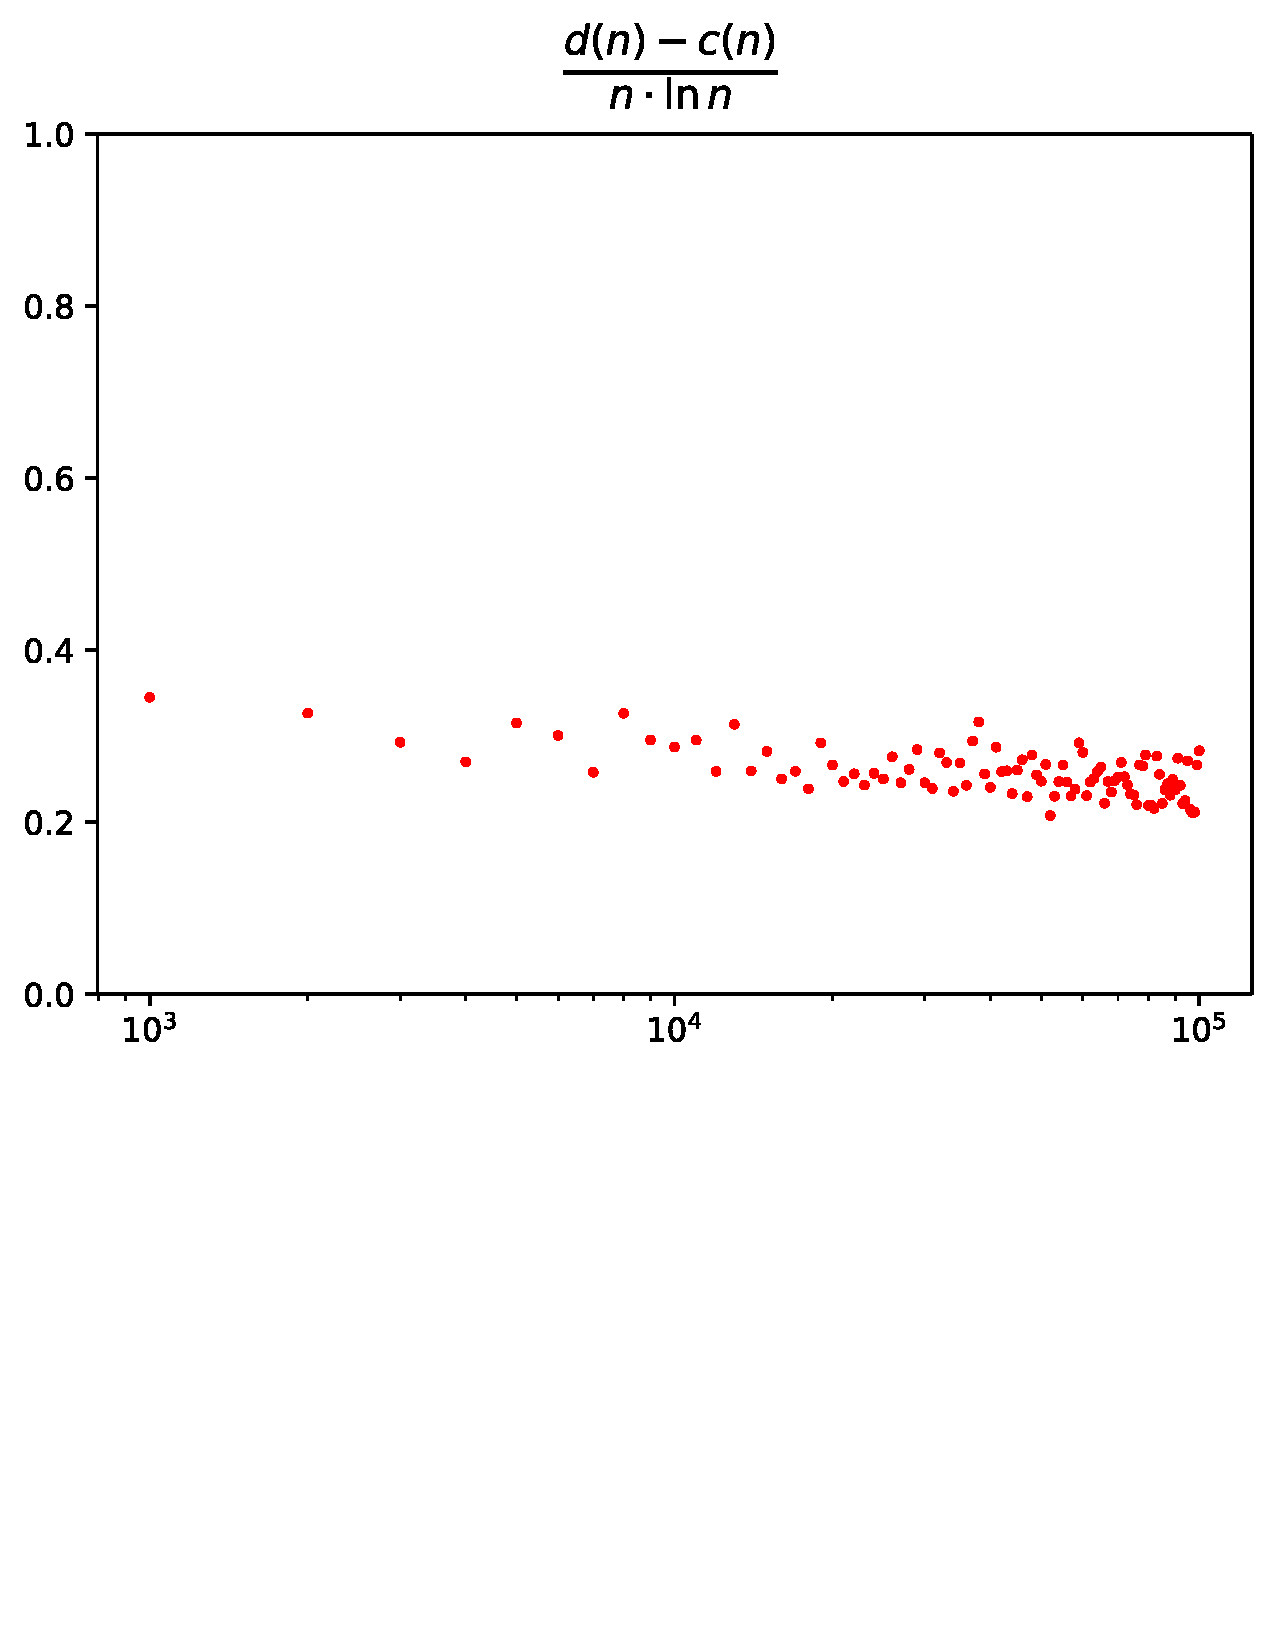
\includegraphics[width=8cm, trim = 0 9cm 0 0, clip]{images/dn-cn2.pdf}
\end{figure}
\begin{figure}[H]
    \centering
    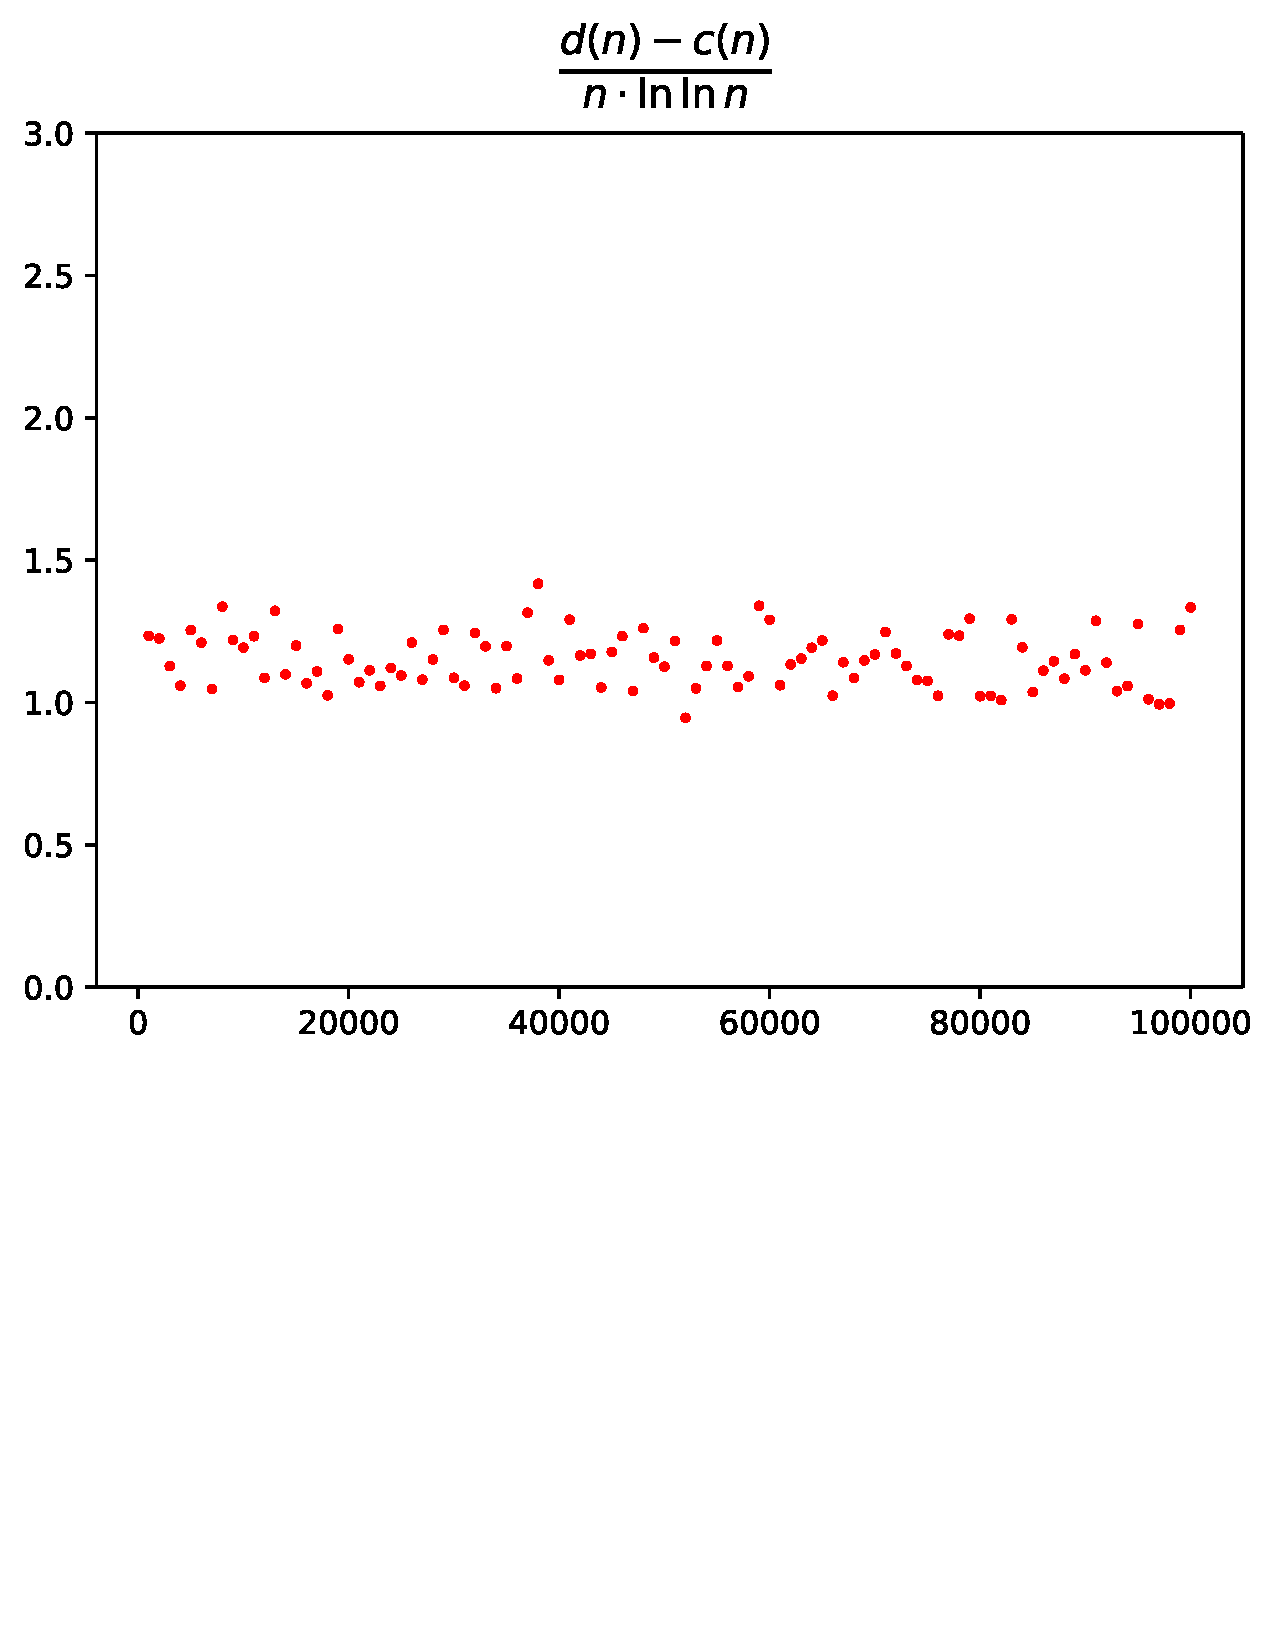
\includegraphics[width=8cm, trim = 0 10cm 0 0, clip]{images/dn-cn3.pdf}
\end{figure}

\section{Wnioski}

Dla każdej z wymienionych na początku wielkości udało się określić asymptotykę. Sprawdzanie ilości urn aż do 100000 było niepotrzebne, ponieważ takie same wnioski można było ustalić dla maksymalnej liczby urn wynoszącej 60000.

\newpage

\section*{Skrypt do rysowania wykresów}

\begin{lstlisting}[language=Python, caption=plot\_graphs.py]
%config InlineBackend.figure_formats = ['svg']
import numpy as np
from matplotlib import pyplot as plt
from math import sqrt, log
        
f = open("results.txt", "r")
lines = f.read().split('\n')
        
conflict_places = np.array([])
avg_conflict_places = np.array([])
        
empty_bins_after_n = np.array([])
avg_empty_bins_after_n = np.array([])
        
max_balls_in_bin = np.array([])
avg_max_balls_in_bin = np.array([])
        
throws_one_ball = np.array([])
avg_throws_one_ball = np.array([])
        
throws_two_balls = np.array([])
avg_throws_two_balls = np.array([])
        
diff_two_one_throws = np.array([])
avg_diff_two_one_throws = np.array([])
        
line_number = 0 # number of line that I read from
        
for n in range(1000, 100000 + 1, 1000):
        
    sum_conflict_place = 0
    sum_empty_bins_after_n = 0
    sum_max_balls_in_bin = 0
    sum_throws_one_ball = 0
    sum_throws_two_balls = 0
    sum_diff_two_one_throws = 0
        
    for k in range(0, 50):
        data = [int(val) for val in lines[line_number].split(';')]
        
        conflict_places = np.append(conflict_places, data[0])
        sum_conflict_place += data[0]
        
        empty_bins_after_n = np.append(empty_bins_after_n, data[1])
        sum_empty_bins_after_n += data[1]
        
        max_balls_in_bin = np.append(max_balls_in_bin, data[2])
        sum_max_balls_in_bin += data[2]
        
        throws_one_ball = np.append(throws_one_ball, data[3])
        sum_throws_one_ball += data[3]
        
        throws_two_balls = np.append(throws_two_balls, data[4])
        sum_throws_two_balls += data[4]
        
        diff_two_one_throws = np.append(diff_two_one_throws, data[5])
        sum_diff_two_one_throws += data[5]
        
    line_number += 1
        
    avg_conflict_places = np.append(avg_conflict_places, sum_conflict_place / 50.0)
    avg_empty_bins_after_n = np.append(avg_empty_bins_after_n, sum_empty_bins_after_n / 50.0)
    avg_max_balls_in_bin = np.append(avg_max_balls_in_bin, sum_max_balls_in_bin / 50.0)
    avg_throws_one_ball = np.append(avg_throws_one_ball, sum_throws_one_ball / 50.0)
    avg_throws_two_balls = np.append(avg_throws_two_balls, sum_throws_two_balls / 50.0)
    avg_diff_two_one_throws = np.append(avg_diff_two_one_throws, sum_diff_two_one_throws / 50.0)
        
f.close()
        
x_axis = [[n for k in range(50)] for n in range (1000, 100000 + 1, 1000)]
x_axis_for_n = range(1000, 100000 + 1, 1000)
        
plt.scatter(x_axis , conflict_places, s = 0.2, color = '#5E81B5')
plt.scatter(x_axis_for_n, avg_conflict_places, s = 4, color = '#FF0000')
plt.title(r'$B_n$', fontsize = 18, pad = 15)
plt.show()
        
plt.scatter(x_axis , empty_bins_after_n, s = 0.2, color = '#5E81B5')
plt.scatter(x_axis_for_n, avg_empty_bins_after_n, s = 4, color = '#FF0000')
plt.title(r'$U_n$', fontsize = 18, pad = 15)
plt.show()
        
plt.hist2d([n for k in range(50) for n in range(1000, 100000 + 1, 1000)], max_balls_in_bin, bins=50, cmap='Blues')
cb = plt.colorbar()
plt.scatter(x_axis_for_n, avg_max_balls_in_bin, s = 4, color = '#FF0000')
plt.title(r'$L_n$', fontsize = 18, pad = 15)
plt.show()
        
plt.scatter(x_axis , throws_one_ball, s = 0.2, color = '#5E81B5')
plt.scatter(x_axis_for_n, avg_throws_one_ball, s = 4, color = '#FF0000')
plt.title(r'$C_n$', fontsize = 18, pad = 15)
plt.show()
        
plt.scatter(x_axis , throws_two_balls, s = 0.2, color = '#5E81B5')
plt.scatter(x_axis_for_n, avg_throws_two_balls, s = 4, color = '#FF0000')
plt.title(r'$D_n$', fontsize = 18, pad = 15)
plt.show()
        
plt.scatter(x_axis , diff_two_one_throws, s = 0.2, color = '#5E81B5')
plt.scatter(x_axis_for_n, avg_diff_two_one_throws, s = 4, color = '#FF0000')
plt.title(r'$D_n - C_n$', fontsize = 18, pad = 15)
plt.show()
        
plt.scatter(x_axis_for_n,
    [avg_conflict_places[i] / ((i + 1) * 1000) for i in range(0, 100)],
    s = 4, color = '#FF0000')
plt.title(r'$\frac{b(n)}{n}$', fontsize = 18, pad = 15)
plt.show()
        
plt.scatter(x_axis_for_n,
    [avg_conflict_places[i] / sqrt((i + 1) * 1000) for i in range(0, 100)],
    s = 4, color = '#FF0000')
plt.ylim(0, 10)
plt.title(r'$\frac{b(n)}{\sqrt{n}}$', fontsize = 18, pad = 15)
plt.show()
        
plt.scatter(x_axis_for_n,
    [avg_empty_bins_after_n[i] / ((i + 1) * 1000) for i in range(0, 100)],
    s = 4, color = '#FF0000')
plt.ylim(0.3, 0.4)
plt.title(r'$\frac{u(n)}{n}$', fontsize = 18, pad = 15)
plt.show()
        
plt.scatter(x_axis_for_n,
    [avg_max_balls_in_bin[i] / log((i + 1) * 1000) for i in range(0, 100)],
    s = 4, color = '#FF0000')
plt.title(r'$\frac{l(n)}{\ln n}$', fontsize = 18, pad = 15)
plt.show()
        
plt.scatter(x_axis_for_n,
    [avg_max_balls_in_bin[i] / (log((i + 1) * 1000) / log(log((i + 1) * 1000))) for i in range(0, 100)],
    s = 4, color = '#FF0000')
plt.ylim(1, 2)
plt.title(r'$\frac{l(n)}{(\ln n)/\ln \ln n}$', fontsize = 18, pad = 15)
plt.show()
        
plt.scatter(x_axis_for_n,
    [avg_max_balls_in_bin[i] / log(log((i + 1) * 1000)) for i in range(0, 100)],
    s = 4, color = '#FF0000')
plt.ylim(2, 4)
plt.title(r'$\frac{l(n)}{\ln \ln n}$', fontsize = 18, pad = 15)
plt.show()
        
plt.scatter(x_axis_for_n,
    [avg_throws_one_ball[i] / ((i + 1) * 1000) for i in range(0, 100)],
    s = 4, color = '#FF0000')
plt.title(r'$\frac{c(n)}{n}$', fontsize = 18, pad = 15)
plt.show()
        
plt.scatter(x_axis_for_n,
    [avg_throws_one_ball[i] / (((i + 1) * 1000) * log((i + 1) * 1000)) for i in range(0, 100)],
    s = 4, color = '#FF0000')
plt.ylim(0, 2)
plt.title(r'$\frac{c(n)}{n \cdot \ln n}$', fontsize = 18, pad = 15)
plt.show()
        
plt.scatter(x_axis_for_n,
    [avg_throws_one_ball[i] / ((i + 1) * 1000) ** 2 for i in range(0, 100)],
    s = 4, color = '#FF0000')
plt.title(r'$\frac{c(n)}{n^2}$', fontsize = 18, pad = 15)
plt.show()
        
plt.scatter(x_axis_for_n,
    [avg_throws_two_balls[i] / ((i + 1) * 1000) for i in range(0, 100)],
    s = 4, color = '#FF0000')
plt.title(r'$\frac{d(n)}{n}$', fontsize = 18, pad = 15)
plt.show()
        
plt.scatter(x_axis_for_n,
    [avg_throws_two_balls[i] / (((i + 1) * 1000) * log((i + 1) * 1000)) for i in range(0, 100)],
    s = 4, color = '#FF0000')
plt.ylim(0, 2)
plt.title(r'$\frac{d(n)}{n \cdot \ln n}$', fontsize = 18, pad = 15)
plt.show()
        
plt.scatter(x_axis_for_n,
    [avg_throws_two_balls[i] / ((i + 1) * 1000) ** 2 for i in range(0, 100)],
    s = 4, color = '#FF0000')
plt.title(r'$\frac{d(n)}{n^2}$', fontsize = 18, pad = 15)
plt.show()
        
plt.scatter(x_axis_for_n,
    [(avg_throws_two_balls[i] - avg_throws_one_ball[i]) / ((i + 1) * 1000) for i in range(0, 100)],
    s = 4, color = '#FF0000')
plt.ylim(0, 5)
plt.title(r'$\frac{d(n) - c(n)}{n}$', fontsize = 18, pad = 15)
plt.show()
        
plt.scatter(x_axis_for_n,
    [(avg_throws_two_balls[i] - avg_throws_one_ball[i]) / (((i + 1) * 1000) * log((i + 1) * 1000)) for i in range(0, 100)],
    s = 4, color = '#FF0000')
plt.ylim(0, 1)
plt.title(r'$\frac{d(n) - c(n)}{n \cdot \ln n}$', fontsize = 18, pad = 15)
plt.show()
        
plt.scatter(x_axis_for_n,
    [(avg_throws_two_balls[i] - avg_throws_one_ball[i]) / (((i + 1) * 1000) * log(log((i + 1) * 1000))) for i in range(0, 100)],
    s = 4, color = '#FF0000')
plt.ylim(0, 3)
plt.title(r'$\frac{d(n) - c(n)}{n \cdot \ln \ln n}$', fontsize = 18, pad = 15)
plt.show()
\end{lstlisting}

\end{document}